\chapter{Paladin大数据存储与处理的容器云平台和MRWS实验}
提出MRWS调度方案优化OpenShift容器云平台底层容器编排引擎Kubernetes调度流程和调度算法后,需要对其资源利用率和负载均衡性进行评估测试。本章主要实验包括如下几个部分:
\begin{enumerate}[(1)]
	\item 在ContainerCloudSim容器云仿真平台上进行大规模容器应用仿真调度实验、对比Kubernetes默认算法、Random算法和MRWS调度算法在资源利用率和负载均衡性方面的性能。
	\item 基于开源OpenShift Origin搭建开发了Paladin容器云平台,该平台是一个集海量数据存储管理、多计算框架快速部署、调度优化、用户注册、按需服务等多功能的容器云PaaS平台。
	\item 在Paladin开发多种分布式计算框架,将其打包成镜像文件,存储在镜像仓库汇中,用户可以快速构建开发测试环境。
	\item 在Paladin平台上开发MRWS算法的调度器,使用多中计算框架容器应用混合部署测试其性能,并与其他调度算法进行对比。
\end{enumerate}

\section{ContainerCloudSim模拟MRWS调度方案}
实验室基于开源OpenShift Origin开发的容器云PaaS平台是在小规模实际物理机上部署,不能进行调度方案的大规模测试和分析,为了评估方案的性能和可靠性,首先在容器云仿真平台ContainerCloudSim上进行大规模的仿真实验。首先构建仿真实验环境,然后开发Kubernetes默认Default调度算法、Random和MRWS调度算法,使用大规模负载进行测试分析。

\subsection{ContainerCloudSim容器云仿真平台}
\subsubsection{CloudSim云仿真平台}
容器和容器编排技术的逐渐成熟推动了容器云的飞速发展,在计算中心的容器云上为了评测资源调度策略和容器服务性能,一个容器云仿真平台变得异常重要。经过大量测试对比调度方案,不仅可以节约开发时间,也能避免造成资源浪费和减少试错成本。针对每一个调度方案,如果部署大规模容器云平台进行性能分析测试,绝大多数的小公司和开发人员并不具备这种条件。在传统的云计算模式下,应用服务的组成、供应、配置和部署条件较为复杂,当用户需求和系统配置动态变化时,评估一个调度策略以及工作负载是相当困难的,一个优秀的云计算平台模拟器可以很好解决这个问题。一个云平台模拟器通过控制环境变量和重复试验可以加速理论研究和开发过程,根据需求和应用场景不同,各大公司和研究机构推出了一系列的云计算平台仿真工具。

MDCSim是一个全面、灵活、可扩展的多层数据中心模拟器,整个模拟平台分为通信层、内核层和用户层建模,通信层用于模拟模拟集群内部通信、内核层模拟调度和分析系统性能、用户层用于模拟各种应用。该模拟器可以根据底层不同硬件特点进行混合建模,用于评估数据中心的能耗,让用户在保持低功耗的同时实现集群服务性能的提升。GroudSim是一个基于Java的模拟器,用于模拟科学应用在网格和云设施上执行问题,模拟完成后给用户提供了基础的统计和分析功能。NetworkCloudSim用于解决网络模拟问题,弥补其他模拟器对网络细节关注不足,支持MPI和工作流。TeachCloud用于对MapReduce应用建模并集成一个负载生成器,提供图形化的接口和实现定制的网络拓扑结构。CloudSim是墨尔本大学Gridbus项目推出的云计算仿真软件,既能对系统性能和应用服务模拟、仿真、试验,也能评估资源调度策略的优劣。

CloudSim是一个开源的仿真软件,最大特点就是提供一个虚拟化引擎,帮助数据中心建立和管理各种虚拟化服务。支持大规模云计算资源管理和调度模拟,将数据中心的资源虚拟化为资源池,CloudSim的分层体系架构图如5.1所示。
\begin{figure}[H] % use float package if you want it here
	\centering
	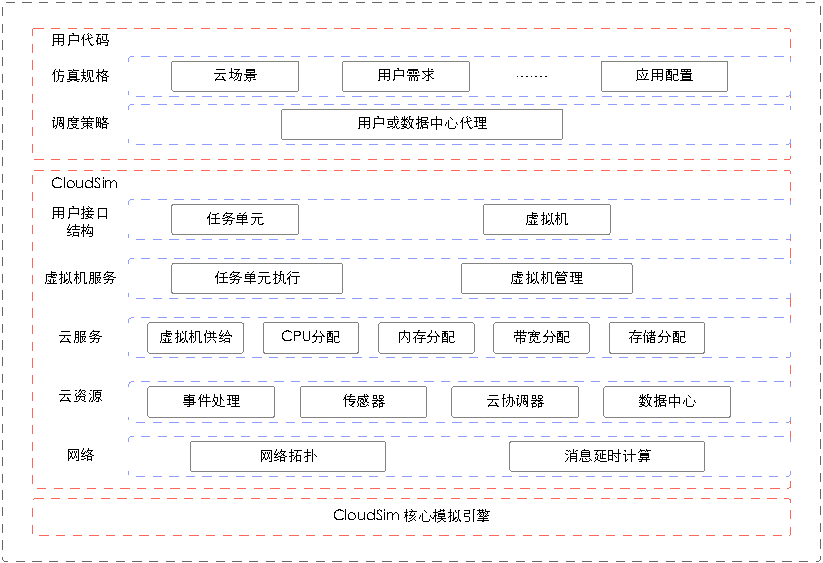
\includegraphics{cloudsim-layer}
	\caption{CloudSim分层架构图}
	\label{fig:xfig1}
\end{figure}

CloudSim是一个分层构建的体系结构,从下到上一次为CloudSim核心引擎层、网络、云资源、云服务、虚拟服务、用户接口结构、资源调度以及仿真规格层。下面一次介绍各层次的大致作用:
\begin{enumerate}[(1).]
	\item CloudSim核心引擎层是离散数据模拟引擎SimJava,为上层提供系统组件构建如服务、数据中心、客户端、代理、虚拟机等,查询和时间处理、通信、模拟时钟等功能。
	\item Network层模拟网络组件如资源收集、数据集、负载测试、信息服务等,对网络设施建模,支持高层软件组件。
	\item 云资源层主要是Host主机和数据中心,主机的核心硬件设施通过数据中心类建模,处理服务请求,构成虚拟资源池。
	\item 云服务层给客户端分配特定应用的VM,同时给VM分配处理内核、内存、磁盘以及网络带宽,可以执行用户新的VM提供策略,有助于一定目标优化。
	\item 虚拟机服务层提供任务执行和虚拟机管理,定义一系列虚拟机创建、销毁、合并、迁移等操作管理,执行基于云环境的应用服务。
	\item 用户接口层向用户提供VM任务单元和虚拟机,将下层的虚拟资源打包成虚拟机提供给用户。
	\item 用户代码层是用户根据实际应用场景和需求,定制应用的规格和调度策略,将应用加入数据中心的代理中,按照资源调度策略进行调度。
\end{enumerate}
CloudSim有一些重要的类和核心概念,针对这些类的大致作用进行简单的介绍:
\begin{enumerate}[1.]
	\item DataCenter类封装底层的Host主机,提供虚拟化的资源,保证每个数据中心至少存在一台运行的Host主机,同时提供虚拟化网络并内置了一个调度组件,为虚拟机和主机分配CPU、内存、网络带宽等资源。
	\item DataCenterBroker类是数据中心代理,负责虚拟机和云任务列表的提交。
	\item VM类是虚拟机类,运行在Host上,多个VM共享Host资源。
	\item Cloudlet类是云任务类,根据用户的设置构建云计算和调度任务。
	\item VmAllocationPolicy类是虚拟机分配策略类,该类实现了虚拟机分配给Host主机的调度策略,用户可以重写该分配策略。
	\item CloudletScheduler类实现多种分配策略,虚拟机内部应用共享处理器的策略,时间共享还是空间共享。
\end{enumerate}

此外,CLoudSim还有数据中心资源配置类DataCenterCharacteristics、扩展虚拟机分配策略的主机类Host、带宽分配策略类BwProvisioner、模拟网络延时行为类NetworkTopology、模拟存储区域网类SanStorage、虚拟分配主存类RamProvisioner、云协调器类CloudCoordinator等一些列重要的类,共同完成CloudSim功能。

\subsubsection{ContaienrCloudSim容器云仿真平台}
随着容器技术的迅猛发展,CaaS(Congtianer as a Service)作为一种新型的服务模式变得越来越普遍。上述介绍的各种云计算仿真平台以及早期的CloudSim版本并不支持容器仿真,一个支持容器应用仿真的平台变得越加紧迫。为了缩短容器云上新方法的开发时间,墨尔本大学的研究人员利用CloudSim虚拟化的特点,在其基础上开发了ContainerCloudSim,专门用于数据中心容器应用的模拟。在最新的CloudSim-4.0上已经集成ContainerCloudSim,提供Docker容器应用仿真支持,ContainerCloudSim与CloudSim生态圈关系如图5.2所示。
\begin{figure}[H] % use float package if you want it here
	\centering
	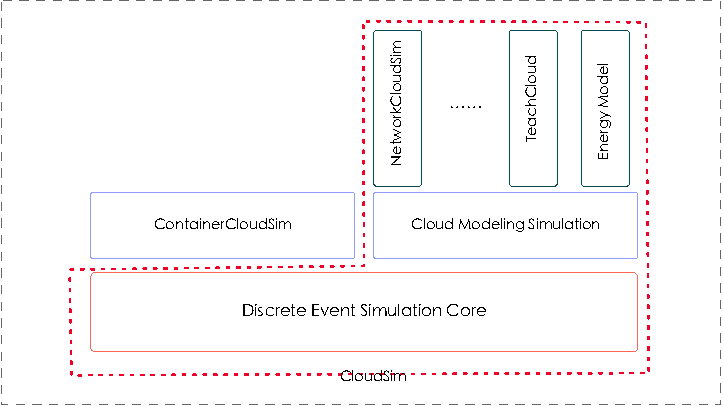
\includegraphics{container-cloudsim}
	\caption{ContainerCloudSim与CloudSim生态圈}
\end{figure}
集成ContainerCloudSim的CloudSim-4.0云平台模拟器已完整支持容器云的仿真,新的版本具有如下几个特点:
\begin{enumerate}[(1)]
	\item 支持数据中心大规模云计算建模和仿真。
	\item 支持服务器虚拟化和主机的建模仿真,定制虚拟机调度策略。
	\item 支持容器应用程序的建模和仿真。
	\item 支持能量感知的计算资源建模和仿真。
	\item 支持网络拓扑结构和消息传递应用建模和仿真。
	\item 支持动态插入元素、停止和恢复的模拟。
	\item 支持混合云的建模和仿真。
\end{enumerate}

在ContainerCloudSim部分,提供容器、VMs、Host、数据中心资源包括CPU、内存和存储的管理功能,实现动态监控系统性、控制容器内应用的执行以及给容器提供虚拟机。容器的模拟器要能给研究人员提供容器调度方案间的对比,容器调度策略决定容器如何被调度到虚拟机上,以及各种调度算法之间的对比和评测。算法的能耗问题也是容器模拟器应该关注的重点,可以提供各种算法的能耗度量,容器的合并和迁移也是模拟器的一大功能。最后,模拟器要能够支持容器的扩展性,在CaaS容器环境中,容器的数量是远远多于虚拟机的。ContainerCloudSim是在CloudSim基础上开发而来,也是一个分层的架构,整体架构如下所示。
\begin{figure}[H] % use float package if you want it here
	\centering
	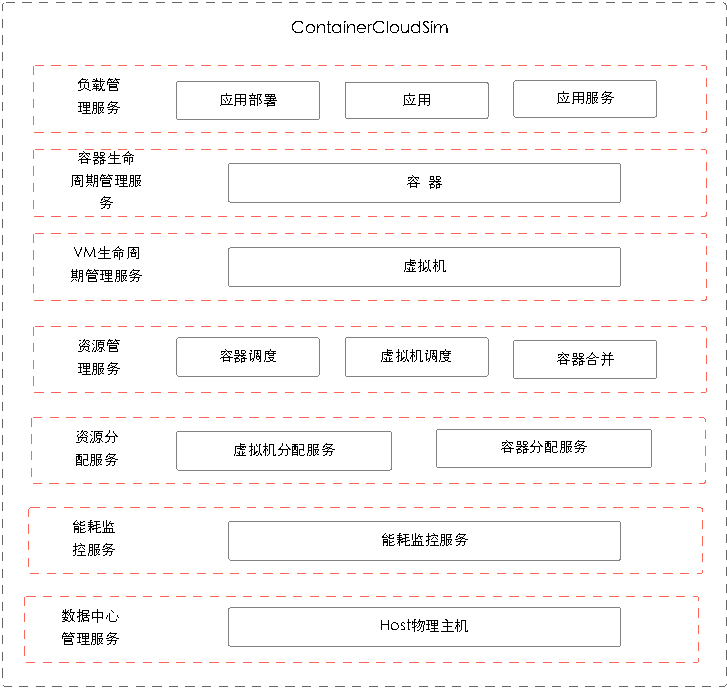
\includegraphics{containercloudsim-layer}
	\caption{ContainerCloudSim分层架构图}
\end{figure}
从底至上依次分为数据中心管理服务、能耗监控服务、资源分配服务、资源管理服务、虚拟机生命周期管理服务、容器生命周期管理服务和负载管理服务等。每个层次的大致作用如下:
\begin{enumerate}
	\item 负载管理服务层关注于客户端应用的注册、部署、调度、应用层级的性能以及应用健康监控。
	\item 容器生命周期服务管理层负责容器生命周期管理,包括创建容器、注册容器到系统中、启动、停止、重启、从一个主机迁移到另一个主机以及容器销毁。除此之外,还负责执行和管理在容器中任务,监控任务资源利用率。
	\item 虚拟机生命周期管理服务层负责虚拟机的管理包括创建、启动、停止、重启、销毁、迁移以及资源利用率监控。
	\item 资源管理服务层负责容器在满足资源需求和软件环境的虚拟机上创建,虚拟机在满足资源需求的主机上创建,由容器调度、虚拟机调度和合并服务构成。容器调度根据容器调度策略调度容器到虚拟机、虚拟机调度根据虚拟机调度策略调度虚拟机到主机,合并策略通过合并容器减少主机需求,最小化资源碎片。
	\item 资源分配层服务管理虚拟机和容器的资源分配,由容器分配服务和虚拟机分配服务构成。容器分配服务负责虚拟机资源分配给容器,虚拟机分配服务负责主机资源分配给虚拟机。
	\item 能耗监控服务负责数据中心主机能耗监控,构建必要的能耗模型。
	\item 数据中心管理服务负责管理数据中心资源,主机开关机以及监控资源利用率。
\end{enumerate}
至此,ContainerCloudSim容器云仿真平台介绍完毕,具体的仿真执行流程具体的实现可以参见其源代码。

\subsection{MRWS资源利用率实验}
在ContainerCloudSim容器云仿真平台上的ContainerPlacementPolicy库下开发MRWS、Kubernetes默认Default算法,该类自带Ramdom算法,对比三种算法下集群资源的利用率。该容器云仿真平台影响调度因素较多,需要根据实际的需要进行一些必要的设置。

首先MRWS算法和Kubernetes的Default算法在预选阶段使用的筛选规则相同,评分阶段除空闲资源评分函数和平衡函数外,其他评分函数相同。因此,假设其他评分函数和外部条件都相同的情况下,只需模拟比较MRWS算法和Default算发的空闲资源评分函数。在模拟器设置方面,要对比容器各种调度算法下集群资源的利用率和负载均衡性,对虚拟机的调度策略已有众多的研究,不是本文的研究方向,因此,假设ContainerCloudSim数据中心的单个Host上只运行一个虚拟机,且虚拟机的资源配置和Host主机相同。本文也不对Container的迁移算法做研究,需要在模拟器上设置容器禁止迁移,即不触发迁移阈值。由于只对容器应用调度研究,不执行具体的云任务,不设置容器、虚拟机和主机的PE数。测试负载是基于PlanetLab负载进行的更改,让CPU、内存、磁盘和带宽的利用率从10\%到90\%的随机变化。虚拟机、主机的配置如表5.1所以,CPU的单位是Mips,容器应用根据负载情况随机构建。在云数据中心中,集群通常是异构的,节点拥有资源数量不同,假设存在三种主机,用于模拟异构集群。
\begin{table}[H]
	\centering\dawu[1.3]
	\caption{主机和虚拟机配置表}
	\begin{tabular}{|p{1.8cm}<{\centering}|p{1.5cm}<{\centering}|p{2cm}<{\centering}|p{1.5cm}<{\centering}|p{1.5cm}<{\centering}|p{1.5cm}<{\centering}|p{1.5cm}<{\centering}|p{1.5cm}<{\centering}|} \hline
		Host类型 & VM类型 & CPU型号 & MIPS & 内存(G) & 磁盘(G) & 带宽(M) \\ \hline
		\#1 & \#1 & i7 7500U & 49360 & 16 & 1000  & 100 \\ \hline
		\#2 & \#2 & i5 8200U & 65770 & 32 & 1000 & 100 \\ \hline
		\#3 & \#3 & X6 1100T & 78440 & 16 & 1000 & 100 \\ \hline
	\end{tabular}
\end{table}

容器应用的配置根据模拟的负载情况自动生成,并对生成的负载自动求解权重参数,参数设置部分代码片段如下:
\begin{lstlisting}[ language=Java]
public static final int VM_TYPES = 3;
public static final double[] VM_MIPS = new double[]{49360, 65770, 78440};
public static final int[] VM_PES = new int[]{};
public static final float[] VM_RAM = new float[] {(float)16000, (float) 32000, (float) 16000};//**MB*
public static final int VM_BW = 100;
public static final int VM_SIZE = 1000000;

public static final int HOST_TYPES = 3;
public static final int[] HOST_MIPS = new int[]{49360, 65770, 78440};
public static final int[] HOST_PES = new int[]{};
public static final int[] HOST_RAM = new int[]{1600,3200,1600};
public static final int HOST_BW = 100;
public static final int HOST_STORAGE = 1000000;

public static final int NUMBER_HOSTS = 30;
public static final int NUMBER_VMS = 30;
public static final int NUMBER_CLOUDLETS = 200;
\end{lstlisting}

模拟实验中设置资源阈值为0.15,一旦节点上的某种资源使用率超过该阈值后将不能部署新的容器应用,模拟实验主要测量在相同数量容器下需要服务器的数量。若节点资源利用越均衡,该节点可部署的容器应用数量越多,从而需要的节点数量越少。实验对比MRWS调度算法、Kubernetes的Default算法简称为KUB算法、Random算法以及FirstFit算法对资源的需求,后两种算法是ContainerCloudSim自带算法,只需要模拟KUB的内存和CPU均衡利用,MRWS综合考虑CPU、内存、磁盘、网络带宽以及已部署Pod应用因素的综合评分算法。模拟实验中单位资源组$res=(cpu,memory,disk,bandwidth)=(10000Mips,4000M,100G,10M)$,单个应用容器的负载是单位资源组的$10\%\sim 90\%$随机变化的资源需求,构建出的应用容器负载如表5.2所示。
\begin{table}[H]
	\centering\dawu[1.3]
	\caption{N个应用容器的资源配置}
	\begin{tabular}{|p{1.8cm}<{\centering}|p{1.8cm}<{\centering}|p{1.8cm}<{\centering}|p{1.8cm}<{\centering}|p{1.8cm}<{\centering}|p{1.8cm}<{\centering}|} \hline
		应用容器 & CPU(MIPS) & 内存(M) & 磁盘(G) & 带宽(M) & Pod \\ \hline
		 1 & 8500 & 680 & 34 & 9 &1 \\ \hline
		 2 & 4000 & 840 & 12 & 16 & 1 \\ \hline
		 3 & 2000 & 3400 & 20 & 6 & 1 \\ \hline
		 4 & 3400 & 1200 & 80 & 10 & 1 \\ \hline
		 ... & ... & ... & ... & ... & ... \\ \hline
		 N & 7600 & 600 & 30 & 4 & 1 \\ \hline
	\end{tabular}
\end{table}
根据MRWS的FAHP自动建模和按照资源需求比值的差值构建模糊成对比矩阵,自动求解容器应用各维度资源的权重参数,上述容器列表各维度资源对应的权重参数如表5.3所示。
\begin{table}[H]
	\centering\dawu[1.3]
	\caption{应用容器资源对应的权重参数表}
	\begin{tabular}{|p{1.8cm}<{\centering}|p{1.8cm}<{\centering}|p{1.8cm}<{\centering}|p{1.8cm}<{\centering}|p{1.8cm}<{\centering}|p{1.8cm}<{\centering}|} \hline
		应用容器 & CPU(MIPS) & 内存(M) & 磁盘(G) & 带宽(M) & Pod \\ \hline
		 1 & 0.528 & 0.086 & 0.136 & 0.214 & 0.036 \\ \hline
		 2 & 0.185 & 0.128 & 0.082 & 0.570 & 0.035 \\ \hline
		 3 & 0.092 & 0.596 & 0.119 & 0.158 & 0.035 \\ \hline
		 4 & 0.140 & 0.095 & 0.508 & 0.221 & 0.036 \\ \hline
		 ... & ... & ... & ... & ... & ... \\ \hline
		 N & 0.596 & 0.092 & 0.158 & 0.119 & 0.035 \\ \hline
	\end{tabular}
\end{table}
测试在相同容器应用数量的条件下所需虚拟机的数量,根据前面一个主机Host上只运行一个和主机配置相同虚拟机,因此虚拟机的数量也是Host主机的数量。实验开始时给定一定数量的Host,三种类型Host数量相同,一旦出现所有主机都无法满足新的容器资源需求,同时增加三种类型Host一台。如200个应用容器时先给定18台主机,以后每次各类型增加一台,即每次增加三台主机,避免某一类型的主机数量过多,测试结果如表5.4所示。
\begin{table}[H]
	\centering\dawu[1.3]
	\caption{相同容器数量下各算法所需主机数}
	\begin{tabular}{|p{1.8cm}<{\centering}|p{1.5cm}<{\centering}|p{1.5cm}<{\centering}|p{1.5cm}<{\centering}|p{1.5cm}<{\centering}|p{1.5cm}<{\centering}|p{1.5cm}<{\centering}|} \hline
		\diagbox[innerwidth=1.8cm]{算法}{容器数} & 200 & 400 & 600 & 800 & 1000 & 1200 \\ \hline
		MRWS & 21 & 42 & 60 & 78 & 96 & 114 \\ \hline
		KUB & 21 & 45 & 69 & 87 & 105 & 129 \\ \hline
		Random & 24 & 48 & 72 & 93 & 117 & 139 \\ \hline
		FirstFit & 27 & 54 & 81 & 108 & 138 & 162 \\ \hline
	\end{tabular}
\end{table}
从上表5.4可以得出,在应用容器数量集群规模较小的情况下,各种算法对主机数量需求相差不大,MRWS调度算法的优势并不明显。这是由于集群中节点各维度资源过载现象较少,整体集群的资源利用率不也高。随着容器数量和主机数量的增加,Random和FirstFit算法劣势越加明显,相同数量下所需的主机数量更多,这是由于随机调度和首个合适节点调度方法容易造成大量相同密集型的应用部署到同一个节点,从而使某一维度资源过载,不能部署更多的应用。Kubernetes的Default算法考虑了CPU和内存的均衡性,其效果比其他两种算法要好,MRWS调度算法综合考虑了各维度资源的均衡性,其效果最佳,所需主机数量最少。MRWS还考虑节点已部署Pod因素,在资源利用率相差不大的情况下避免某个节点部署大量较小资源需求的容器应用,给节点容器管理造成过大开销,从而降低集群性能。容器应用应该分散和均衡地部署到集群的各节点上,提升集群服务性能。

\subsection{MRWS负载均衡实验}
集群服务性能一个关键问题就是负载均衡,而调度策略是影响负载均衡的核心因素。好的负载均衡策略不仅可以提升集群负载处理能力,缩短任务执行时间,也能有效避免单点故障。当前服务器的负载均衡算法一般有随机算法、轮询和加权轮询、最小连接和加权最小连接、哈希算法、IP散列法以及URL散列等。一些重用的负载均衡组件有Apache、Nginx、LVS(Linux Virtual Server)、HAproxy、KeepAlived、Memcached等。Apache和Nginx是一个HTTP的服务器,具有反向代理能力,通过对用户请求分流实现负载均衡;LVS是一个虚拟的服务器集群系统,可以实现Linux平台下简单的负载均衡;HAproxy提供高可用、负载均衡以及基于TCP和HTTP代理,适用于负载较大的web服务站点;KeepAlived也是一个组件,用于检测服务集群中故障节点,及时处理不健康的节点;Memcached是内存缓存系统,对于业务查询数据进行缓存,降低节点的负载,也是一个负载均衡组件。本文主要研究集群中各节点多维资源负载情况,目的在于新的调度方法是否具有更好的资源负载,各维度资源利用是否更加均衡。实验将从三个方面进行对比MRWS算法、Kubernetes的Default算法、Random算法和FirstFit算法中单个节点的相同维度资源、单个节点各维度资源均值、整个集群负载均衡性进行对比,评价指标如式(3-10、3-11)所示。测试过程中假定集群数量、应用容器数量不同的条件下上述三个指标的负载不均衡度。

首先测试集群中各节点某个维度资源利用均衡情况,希望集群中节点上某个维度资源如CPU利用率更加平滑,若节点上该维度资源波动过大则表明其服务性能可能会降低,下面以CPU为例,其他维度资源类似。
\begin{figure}[h]
	\centering%
	\begin{subfigure}{7cm}
		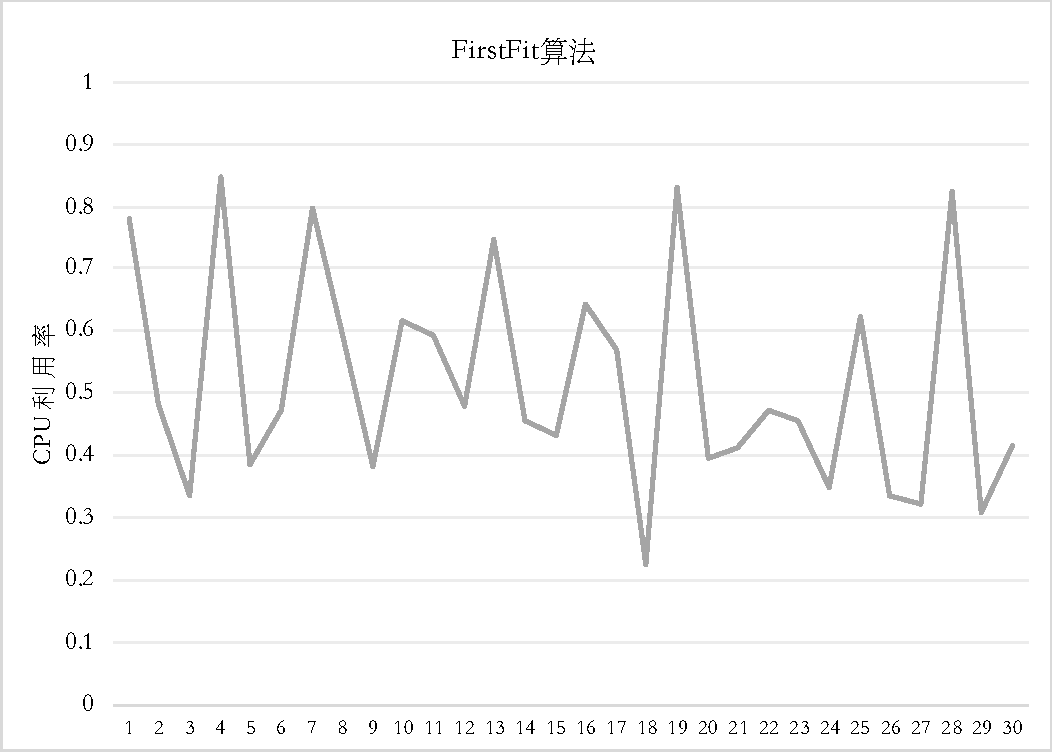
\includegraphics[width=7cm,height=5cm]{firstfit-cpu}
		\caption{FirstFit算法CPU利用率}
	\end{subfigure}%
	\hspace{0.5cm}%
	\begin{subfigure}{7cm}
		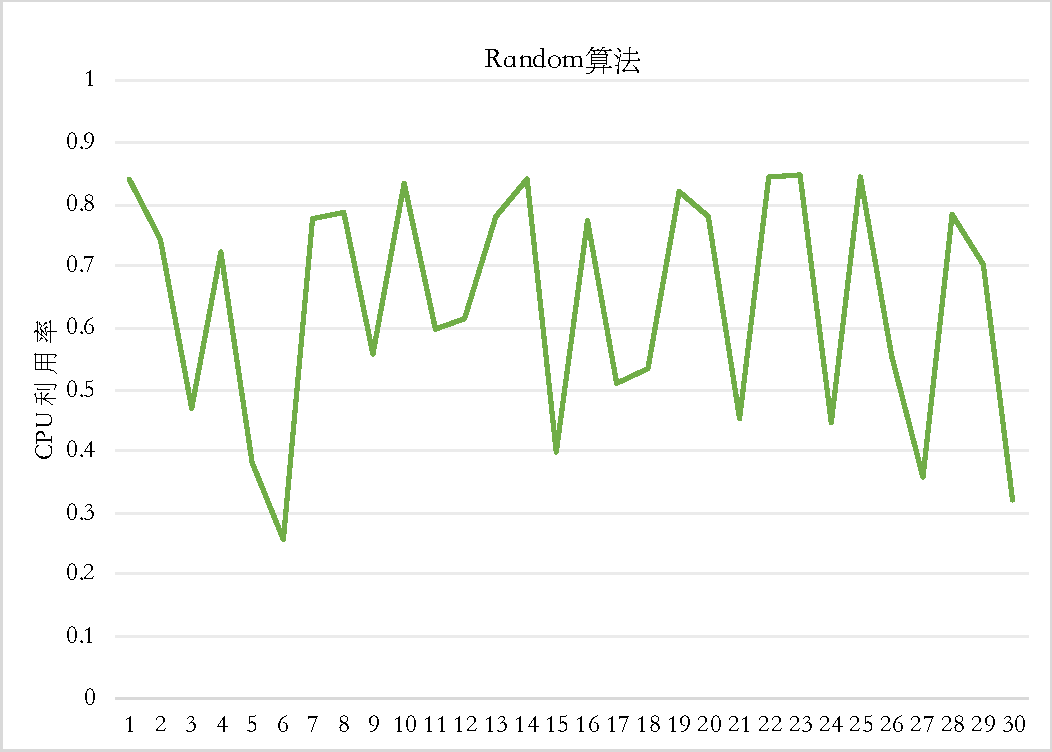
\includegraphics[width=7cm, height=5cm]{random-cpu}
		\centering{\caption{Random算法CPU利用率}}
	\end{subfigure}
	\begin{subfigure}{7cm}
		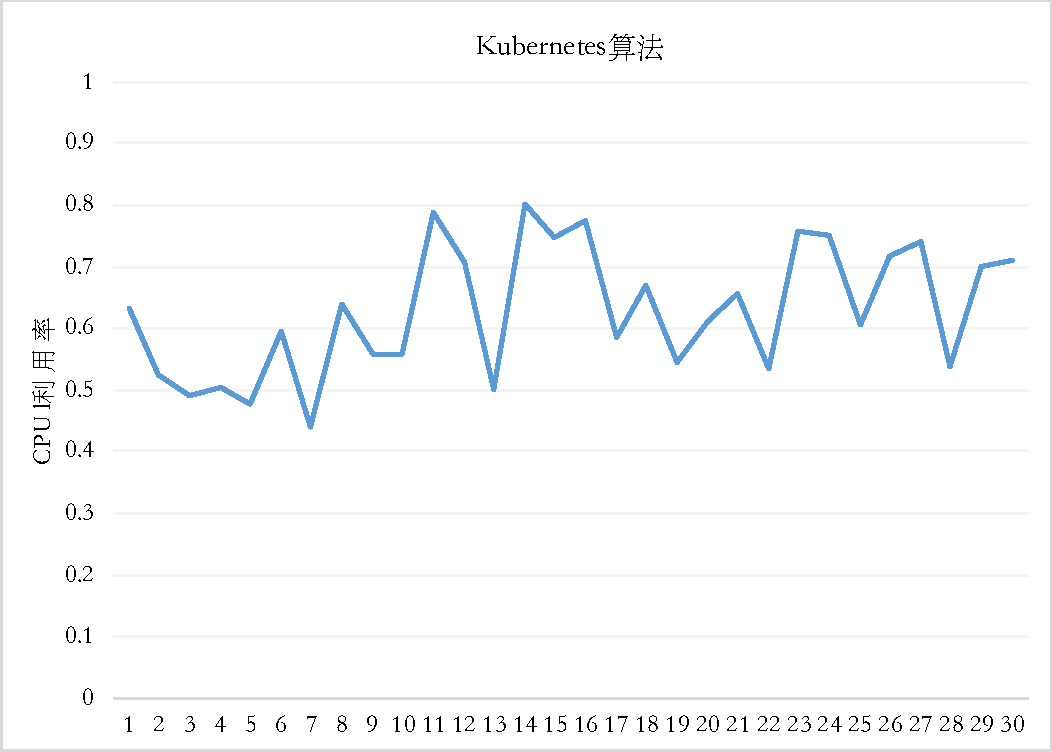
\includegraphics[width=7cm,height=5cm]{kub-cpu}
		\caption{kubernetes算法CPU利用率}
	\end{subfigure}%
	\hspace{0.5cm}%
	\begin{subfigure}{7cm}
		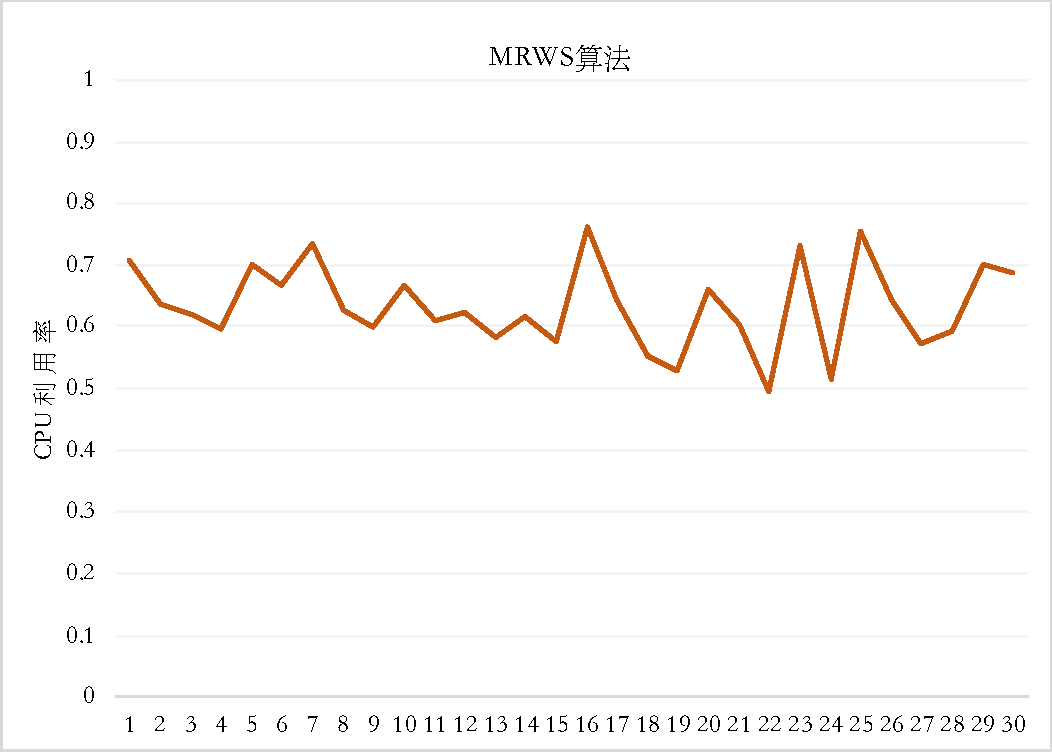
\includegraphics[width=7cm, height=5cm]{mrws-cpu}
		\centering{\caption{MRWS算法CPU利用率}}
	\end{subfigure}
	\caption{四种调度算法下节点CPU利用率波动图}
	
\end{figure}

从图5.4看出,MRWS调度算法下CPU利用率波动性较小,Kubernetes调度算法次之,Random和FirstFit算法节点CPU利用率波动较大。这是由于前两种算法都考虑了CPU利用的均衡性,其中Kubernetes在进行节点评分时考虑了CPU和内存平衡利用,MRWS调度算法综合考虑了CPU、内存、磁盘、网络带宽和已部署的Pod的因素。有效避免单个节点某个维度资源资源利用过高,出现过载现象,从而不能调度更多的应用,造成其他维度的资源浪费,MRWS算法能够有效提升集群的服务性能和资源利用率。下面的实验使用之前定义的均衡度对集群中单个节点上资源均衡度进行测量,实验中假设应用容器数量相同,分别用四种算法对其进行调度,计算单个节点的负载均衡度,部分节点的负载均衡度如下。

\begin{figure}[H]
	\centering%
	\begin{subfigure}{7cm}
		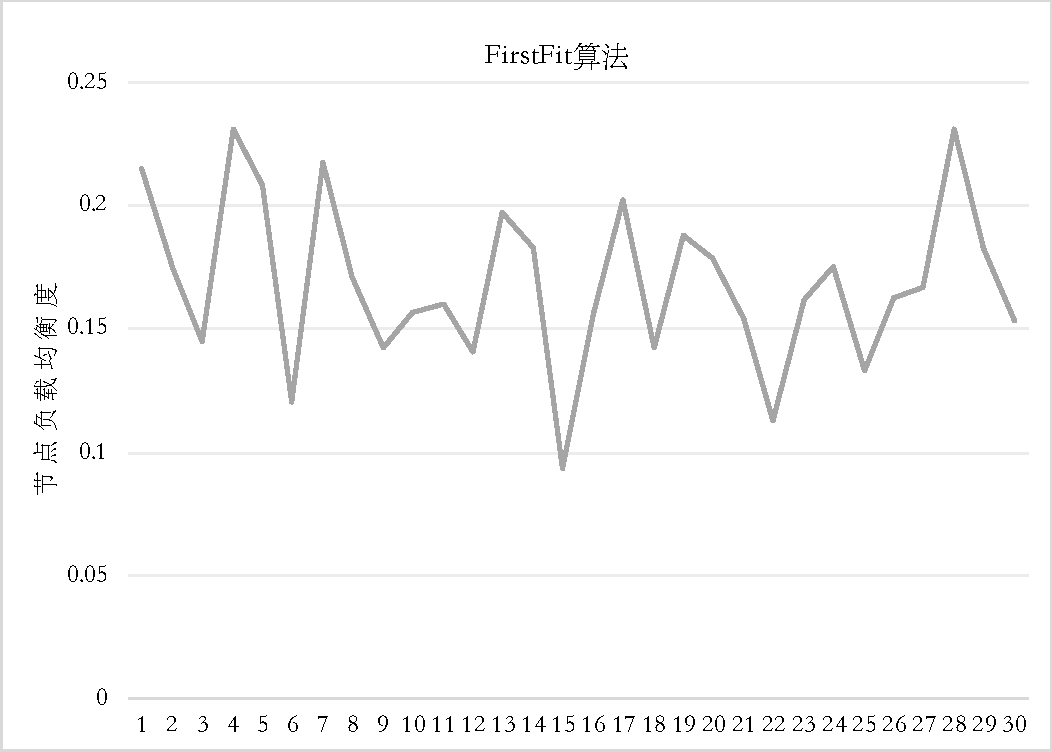
\includegraphics[width=7cm,height=5cm]{firstfit-ba}
		\caption{FirstFit算法节点负载均衡度}
	\end{subfigure}%
	\hspace{0.5cm}%
	\begin{subfigure}{7cm}
		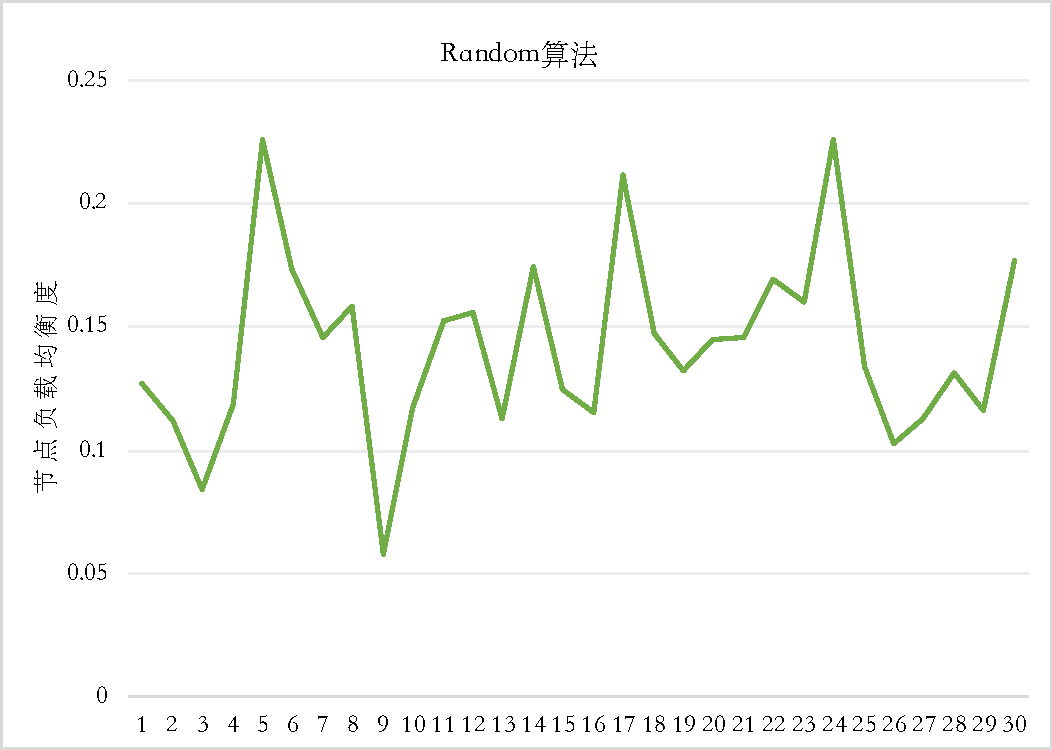
\includegraphics[width=7cm, height=5cm]{random-ba}
		\centering{\caption{Random算法节点负载均衡度}}
	\end{subfigure}
	\begin{subfigure}{7cm}
		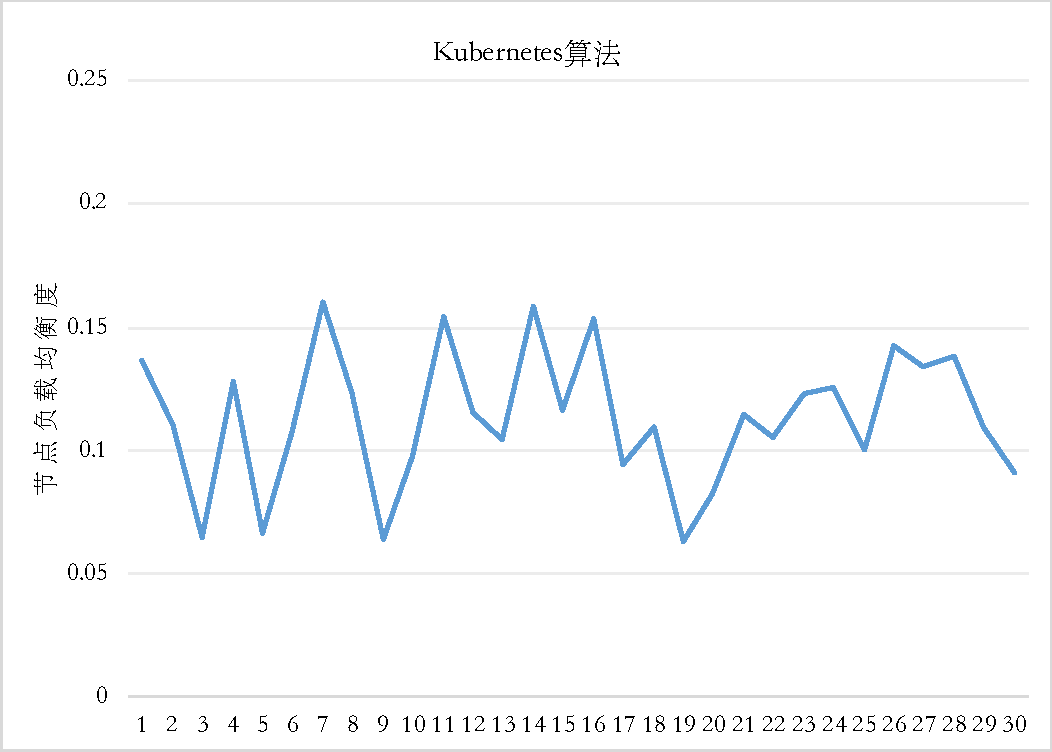
\includegraphics[width=7cm,height=5cm]{kub-ba}
		\caption{kubernetes节点负载均衡度}
	\end{subfigure}%
	\hspace{0.5cm}%
	\begin{subfigure}{7cm}
		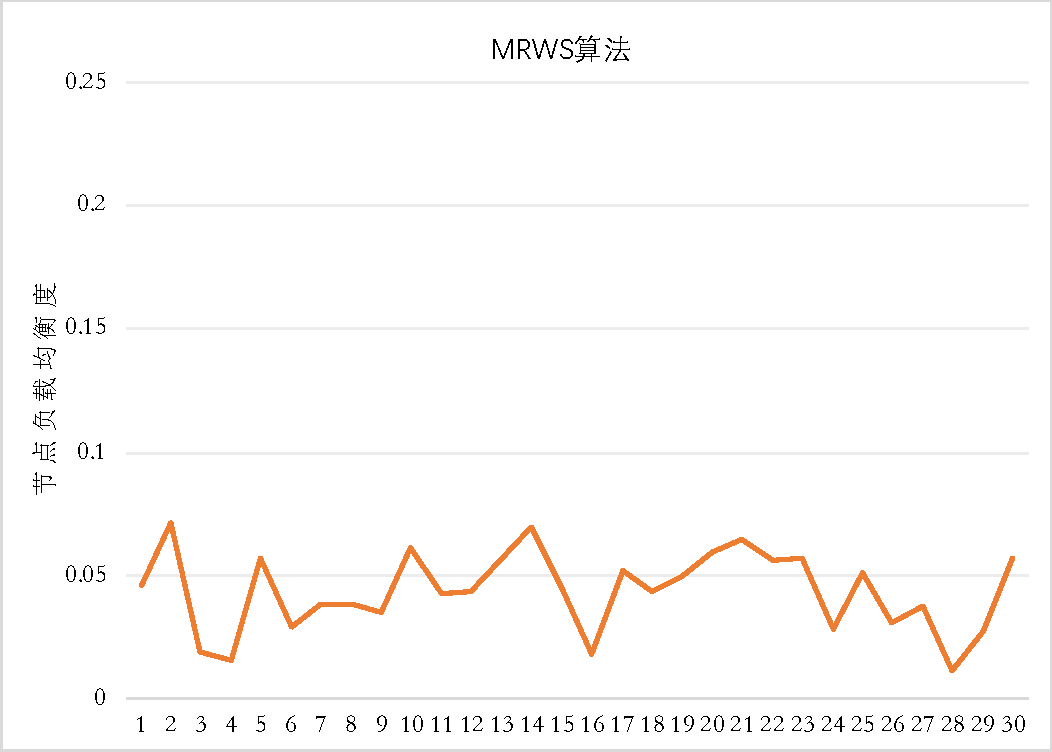
\includegraphics[width=7cm, height=5cm]{mrws-ba}
		\centering{\caption{MRWS算法节点负载均衡度}}
	\end{subfigure}
	\caption{四种调度算法下节点负载均衡度}
	
\end{figure}

如图5.5所示,四种调度算法中MRWS算法的负载均衡度最小,且波动也最小,Kubernetes算法次之,Random和FirstFit算法节点的负载均衡度波动最大并且节点负载均衡度较大。负载均衡度反映节点上各位资源空闲率的均衡程度,负载均衡度越大,各位资源消耗越不均衡,某个维度资源过载现象越严重。由于Random算法随机选择可用节点,FirstFit算法每次选择第一个满足资源需求的节点,完全不考虑各维资源的空闲情况,导致其负载均衡度较大,节点资源利用不充分。Kubernetes平衡CPU和内存利用率,其效果较另外两种要好,MRWS综合了各维度资源空闲率进行评分,其效果最佳,不仅负载均衡度整体偏小,其波动性也小。

接下来进行四种调度算法下集群负载均衡度的对比,假定在容器应用数量不同的情况下,比较整个集群的负载均衡度情况。应用数量相同,负载均衡度越小,集群中过载的节点数量越少,相同情况下集群服务性能会越好,各维度资源消耗更加均匀,应用的调度更合理。

\begin{figure}[H]
	\centering%
	\begin{subfigure}{7cm}
		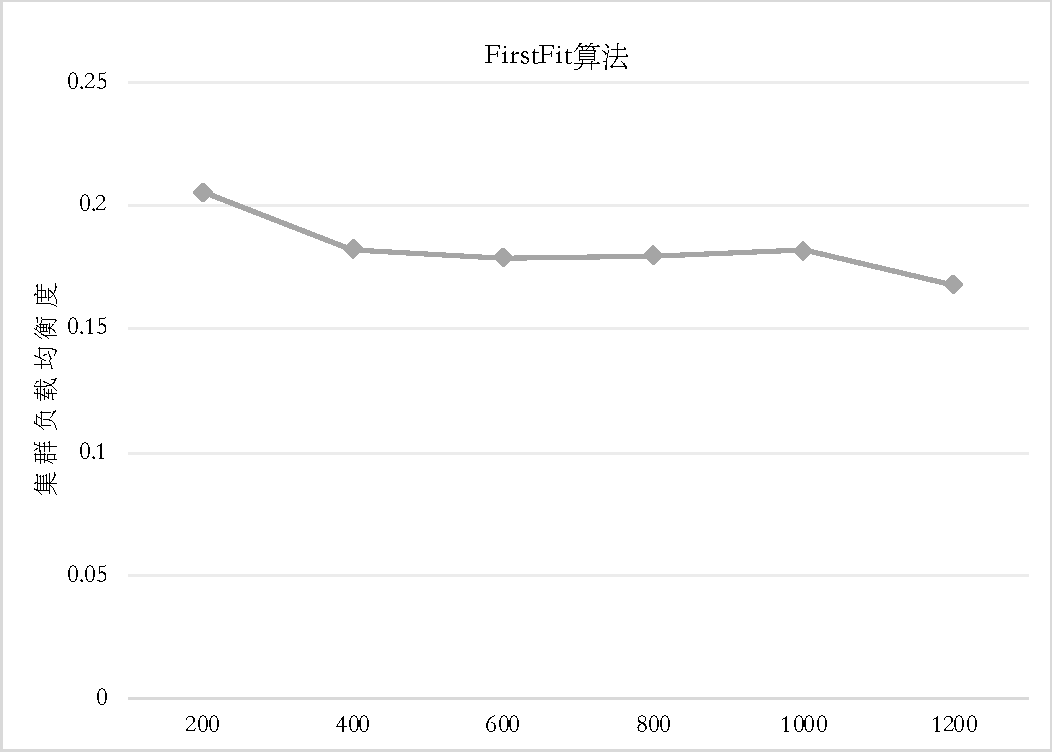
\includegraphics[width=7cm,height=5cm]{firstfit-cluster}
		\caption{FirstFit算法节点负载均衡度}
	\end{subfigure}%
	\hspace{0.5cm}%
	\begin{subfigure}{7cm}
		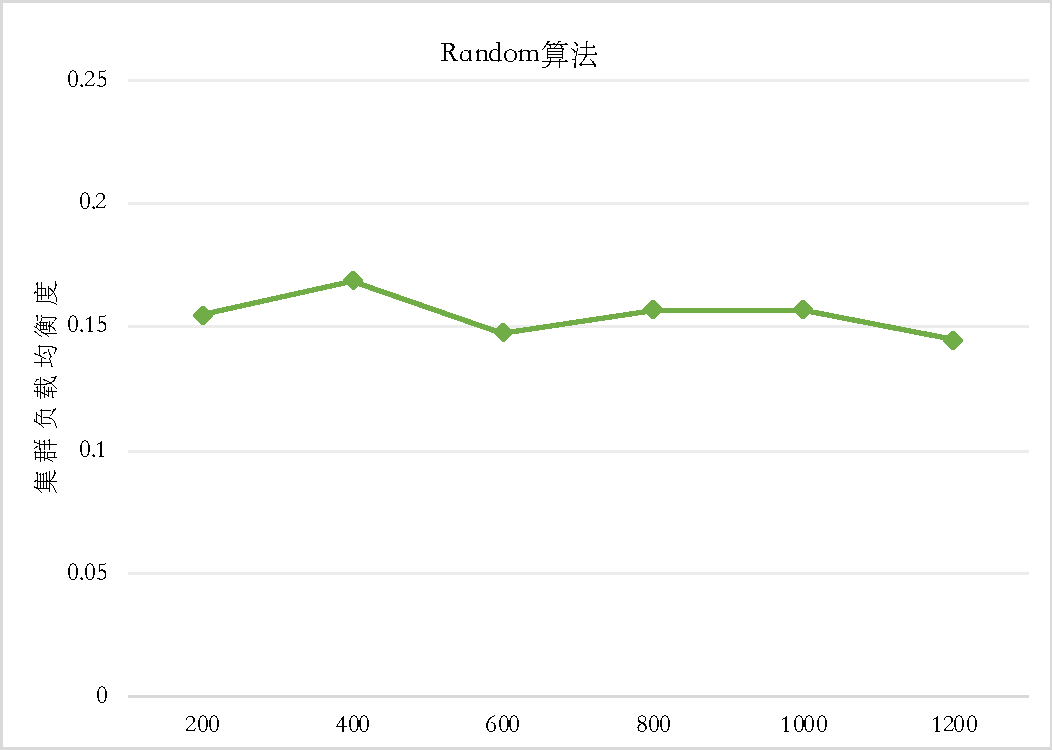
\includegraphics[width=7cm, height=5cm]{random-cluster}
		\centering{\caption{Random算法节点负载均衡度}}
	\end{subfigure}
	\begin{subfigure}{7cm}
		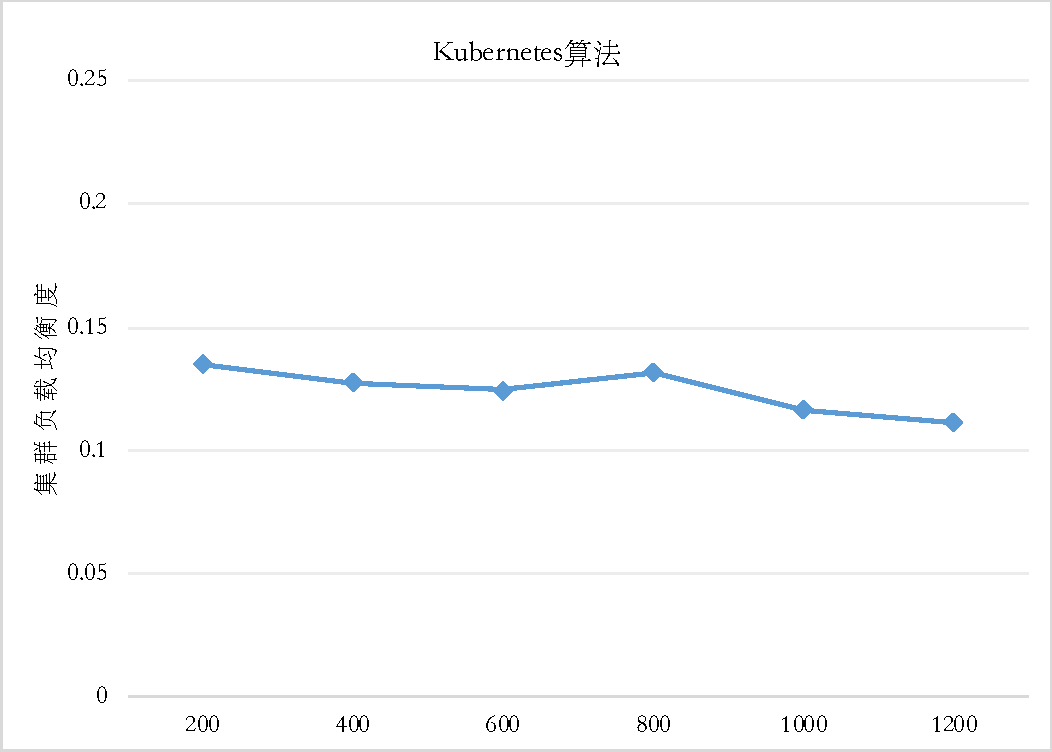
\includegraphics[width=7cm,height=5cm]{kub-cluster}
		\caption{kubernetes节点负载均衡度}
	\end{subfigure}%
	\hspace{0.5cm}%
	\begin{subfigure}{7cm}
		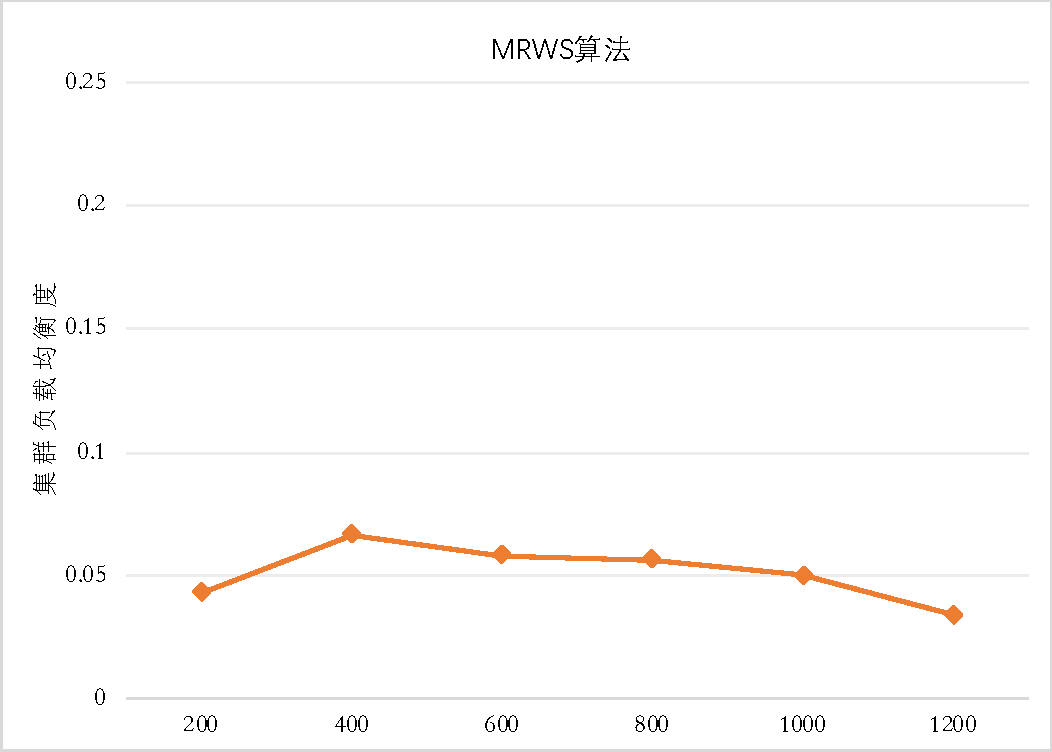
\includegraphics[width=7cm, height=5cm]{mrws-cluster}
		\centering{\caption{MRWS算法节点负载均衡度}}
	\end{subfigure}
	\caption{四种调度算法下集群负载均衡度}	
\end{figure}

如图5.6所示,MRWS调度算法集群的负载均衡度最小,大概为Kubernetes算法的二分之一,Ramdom和FirstFit算法的四分之一。因此,在MRWS调度算法的集群中各节点资源消耗情况趋于均衡,单个节点上各维度资源利用也较为均衡,集群的服务性能更优秀。针对集群的服务性能将使用多计算框架应用混合部署在实际的实验平台上进行测试,测试集中调度算方法下混合应用的完成时间。

\section{Paladin大数据存储与处理的容器云平台部署}
由于不具备大规模实际容器云环境对几种调度算法进行测试,将在实验室小规模容器云平台Paladin上对算法性能进行测试,实验中使用多种分布式计算框架容器应用进行混合部署和性能测试。因此,首先需要搭建一个Paladin实验环境,Paladin是实验室开发的一个集海量数据存储管理,基于容器的多种分布式计算框架运行环境快速构建,存储和计算分离的多元化大数据数据处理平台。
\subsection{Paladin大数据存储与处理的容器云平台介绍}
Paladin是一个支持用户构建多种大数据计算框架、并提供海量数据存储与管理的平台。用户在平台中选择所需的计算与存储框架,如批处理(Hadoop、Spark),流计算系统(Storm、Flink)、分布式的MPI、机器学习框架(Mahout、Tensorflow)、图计算系统(GridGraph、ReGraph)以及数据库系统(MongoDB、Mysql、Redis)等等。平台能够快速构建相应的多计算框架运行环境、并且根据具体的需求提供计算任务调度、海量数据存储,通过优化的容器云多维资源利用率均衡调度算法提升资源利用率和集群服务性能。

\begin{figure}[H] % use float package if you want it here
	\centering
	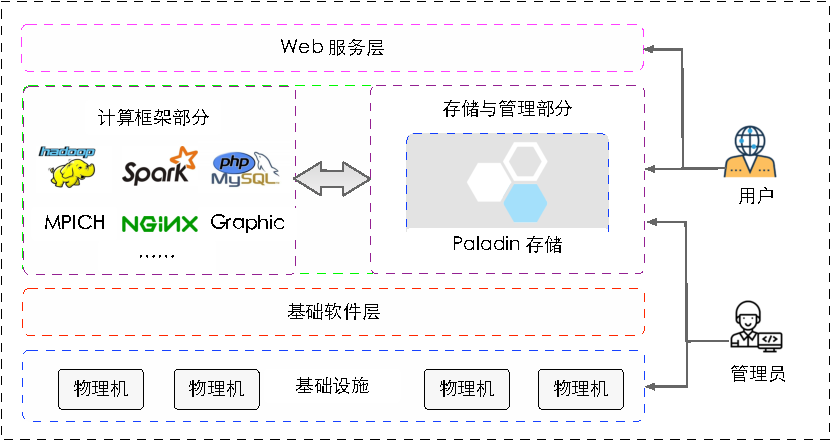
\includegraphics{paladin-structure}
	\caption{Paladin平台架构图}
\end{figure}

从Paladin架构图可以看出,最底层是基础设施部分,即整个集群的物理机和云主机部分,中间是支持上层的中间软件服务如分布式文件系统、Docker容器服务、OpenShift Origin容器云等,最上层提供海量数据存储管理和多种数据处理计算框架,顶层是Web服务层。整个架构中最为重要的两个部分数据存储管理模块和数据处理框架模块,数据管理存储提供用户数据上传、下载、管理、浏览、分享、挂在等一个分布式大数据管理存储系统。数据处理框架提供用户快速构建各种计算框架容器集群环境,根据实际需求配置资源、容器的动态增减变动等,该部分基于开源OpenShift Origin进行搭建,在任何一个容器中可以实现存储数据的挂载,实现存储和计算分离。当前计算框架除支持单应用的Nginx、Apache、PHP、MongoDB等,也支持大量分布式数据处理框架如Hadoop、SPark、Storm、Spark、TensorFlow以及实验室的图计算Regraph、GridGraph等数十种计算框架运行环境的快速部署。用户既可以简单用该系统进行大数据存储管理,也能快速构建大数据处理框架,实现海量数据处理,管理员对基础设施和存储节点,以及系统权限等进行管理。

\subsection{Paladin大数据存储与处理的容器云平台部署}
首先需要构建小规模的Paladin数据存储处理平台,构建一个容器云环境,该平台集成数据存储和管理。实验中采用6台物理机进行部署,一个主节点Matser,Master节点同时也是Node节点,四个Node节点和一个存储Master节点,由于该存储也需要对用户提供Web Service的服务,因此单独使用一个节点进行部署。将用户的存储管理服务和计算框架服务分离,分别部署在两个不同的物理机上,提升集群吞吐率。S-Master是分布式存储的Master节点,各物理节点的配置如下:
\begin{table}[H]
	\centering\dawu[1.3]
	\caption{Paladin平台物理机配置}
	\begin{tabular}{|p{1.8cm}<{\centering}|p{1.5cm}<{\centering}|p{1.5cm}<{\centering}|p{1.5cm}<{\centering}|p{1.5cm}<{\centering}|p{3cm}<{\centering}|} \hline
		\diagbox[innerwidth=1.8cm]{节点}{资源} & CPU核数 & 内存(G) & 磁盘(G) & 带宽(M) & IP \\ \hline
		Master & 4 & 16 & 1000 & 100 & 192.168.1.100  \\ \hline
		Node1 & 4 & 16 & 1000 & 100  & 192.168.1.101 \\ \hline
		Node2 & 4 & 16 & 1000 & 100  & 192.168.1.102 \\ \hline
		Node3 & 4 & 16 & 1000 & 100  & 192.168.1.103 \\ \hline
		Node4 & 4 & 16 & 1000 & 100  & 192.168.1.104 \\ \hline
		S-Matser & 4 & 8 & 500 & 100  & 192.168.1.110 \\ \hline
	\end{tabular}
\end{table}

各节点上需要安装的主要软件如下图所示,部署一个完整的容器云平台。在分布式计算框架部分Master节点上主要部署openshift-ansible及其依赖的各种软件包,用于安装OpenShift集群、openshift-origin集群、底层的Docker及其私有仓库、openshift-origin以来的一致性存储Etcd、实验室数据存储管理需要的哭护短paladin-client、经过优化更改后的origin-web、操作系统Centos 7.5。Master节点即作为容器云的主控节点,同时也是Node节点,在分布式存储中作为数据存储节点。S-Mastershi是分布式存储和管理的主控节点,使用Centos 6.9系统,安装Nginx服务、paladin-web-console对普通用户提供数据存储管理的web服务,同时也是数据节点。Node节点作为计算节点,安装Docker、openshift-origin集群子节点的需要的依赖软件如kublet、Haproxy等系列软件、同时还有Etcd和paladin-client、作为存储集群的数据节点,系统是Centos7.5。
\begin{figure}[H] % use float package if you want it here
	\centering
	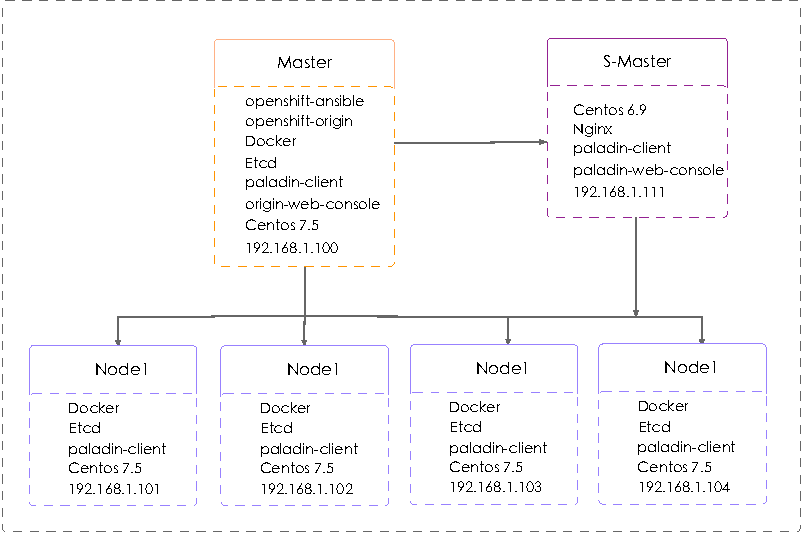
\includegraphics{paladin-platform}
	\caption{Paladin平台节点分布图}
\end{figure}

安装完成后,Paladin平台的计算框架部分,查询集群活跃节点如下:
\begin{figure}[H] % use float package if you want it here
	\centering
	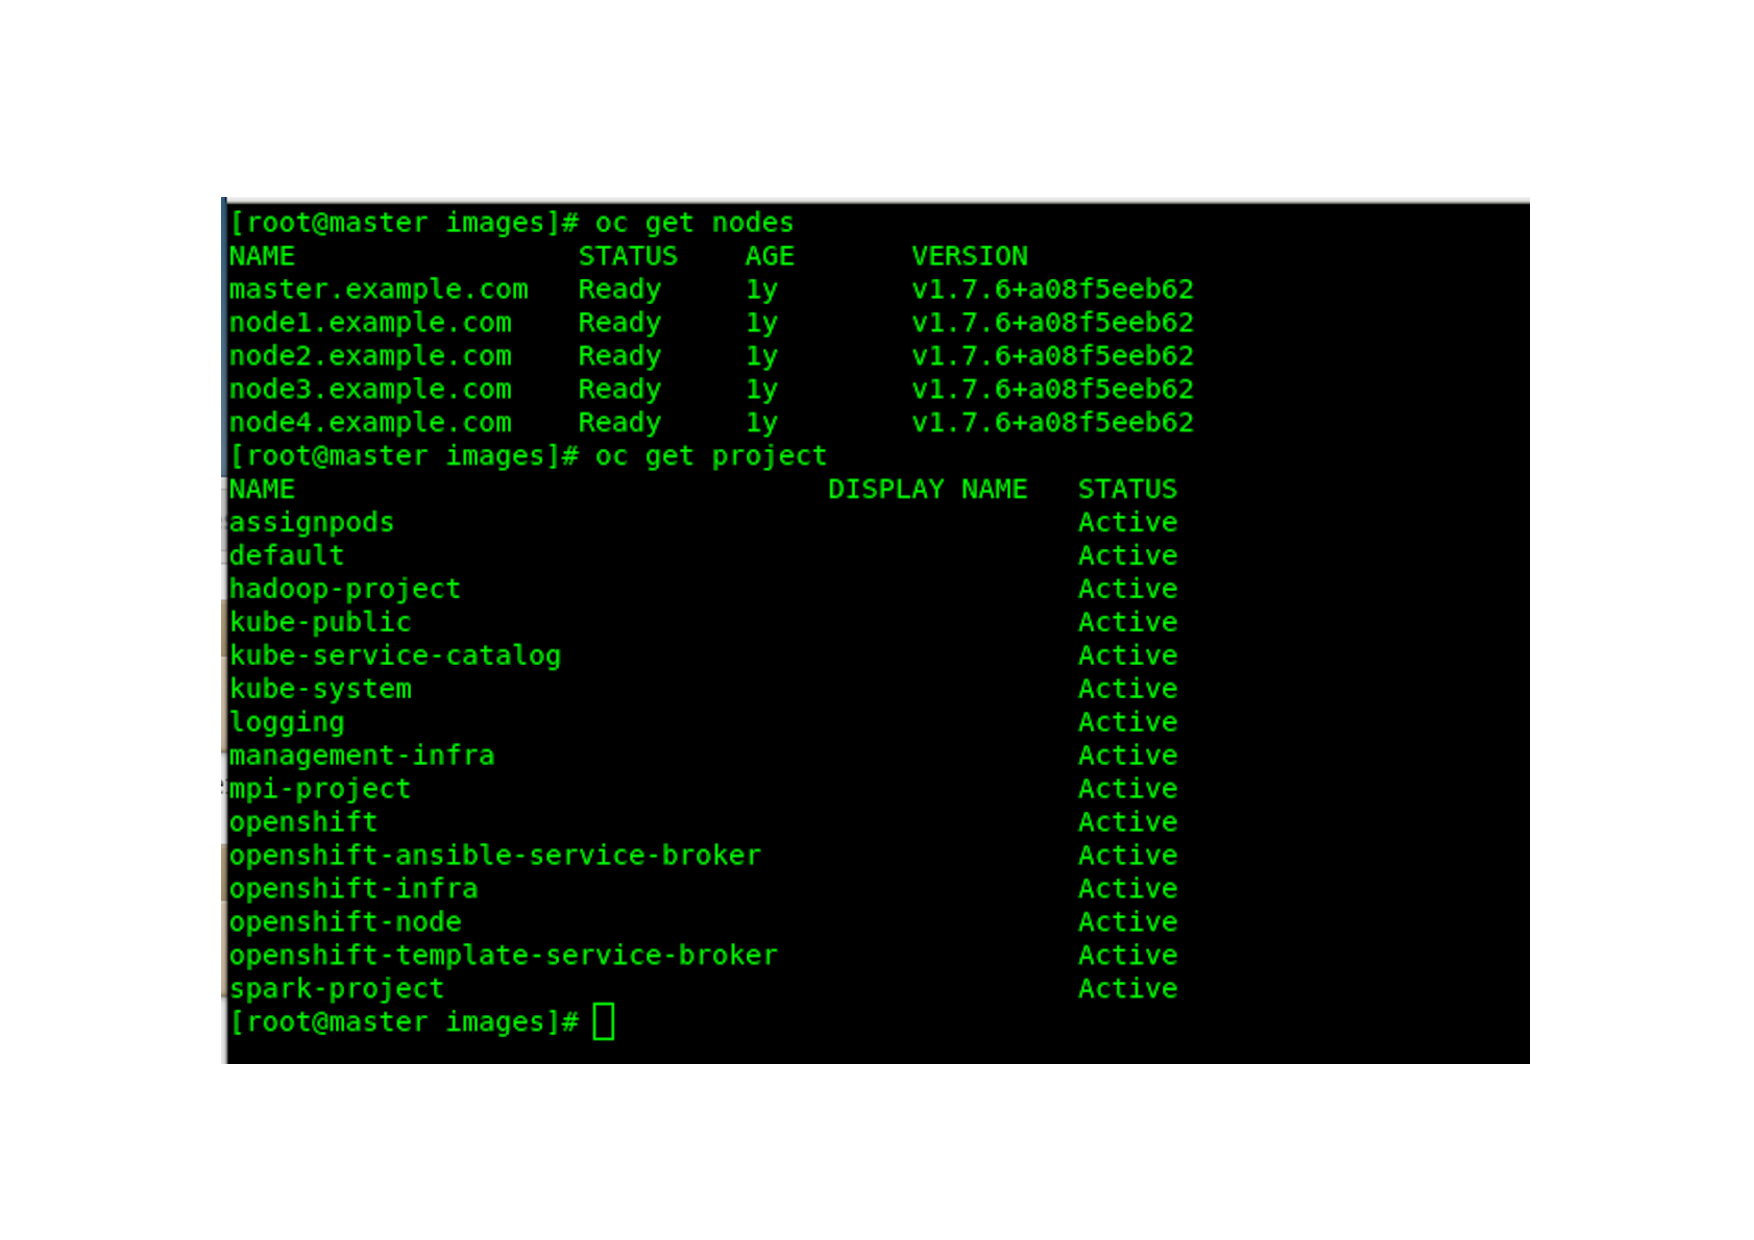
\includegraphics[width=13cm, height=8cm]{paladin-nodelist}
	\caption{Paladin安装成功计算节点部分}
\end{figure}

存储paladin-web-console部分,用户进行数据存储管理,用户在该部分可以进行海量数据的上传、下载、删除等管理,还可以通过paladin-client将数据以盘的形式挂在到物理节点或者容器中,在分布式计算框架容器应用中直接使用数据,实现存储和计算分离。
\begin{figure}[H] % use float package if you want it here
	\centering
	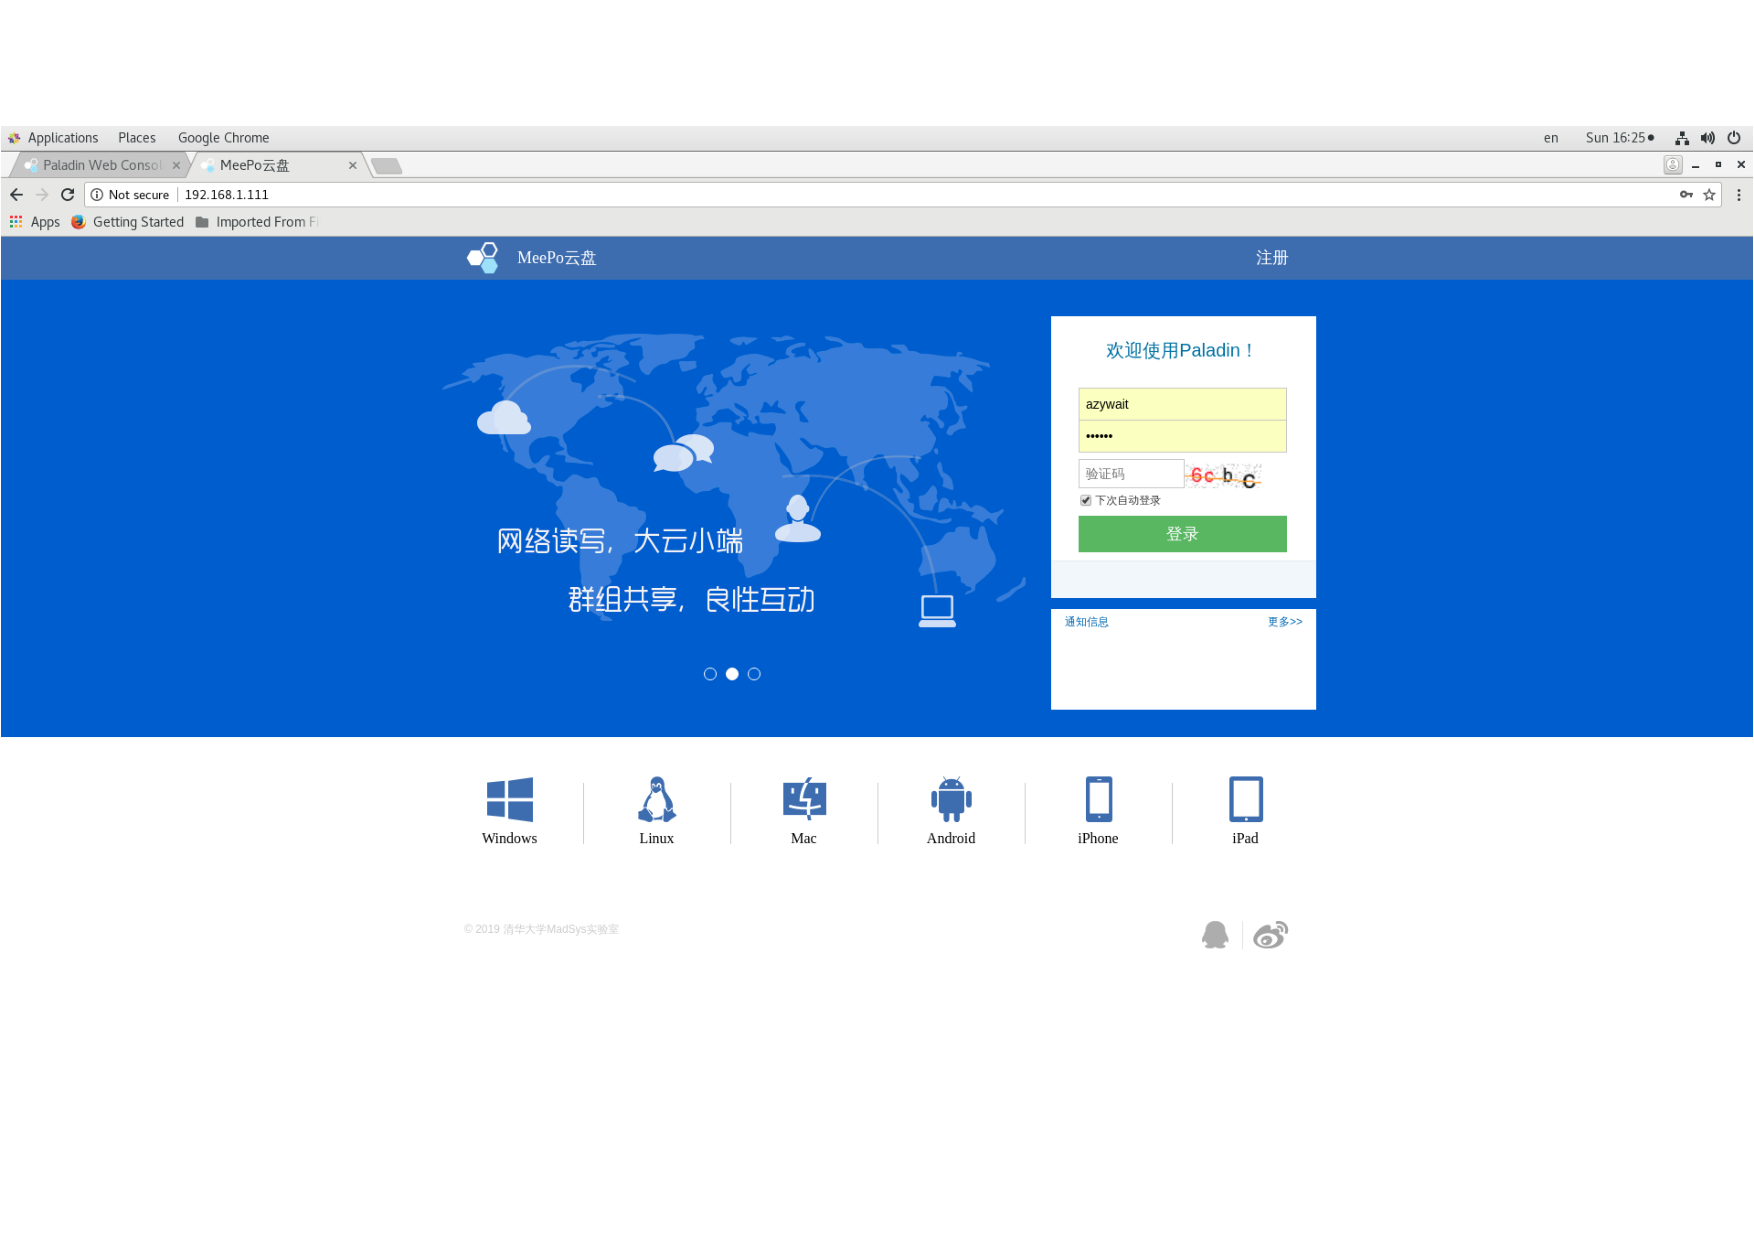
\includegraphics[width=13cm, height=7cm]{paladin-web-console}
	\caption{Paladin数据存储管理服务}
\end{figure}

整个Paladin平台部署完成后,在该平台上开发部署各种大数据处理框架和容器应用,平台origin-web-console用户服务界面如下:
\begin{figure}[H] % use float package if you want it here
	\centering
	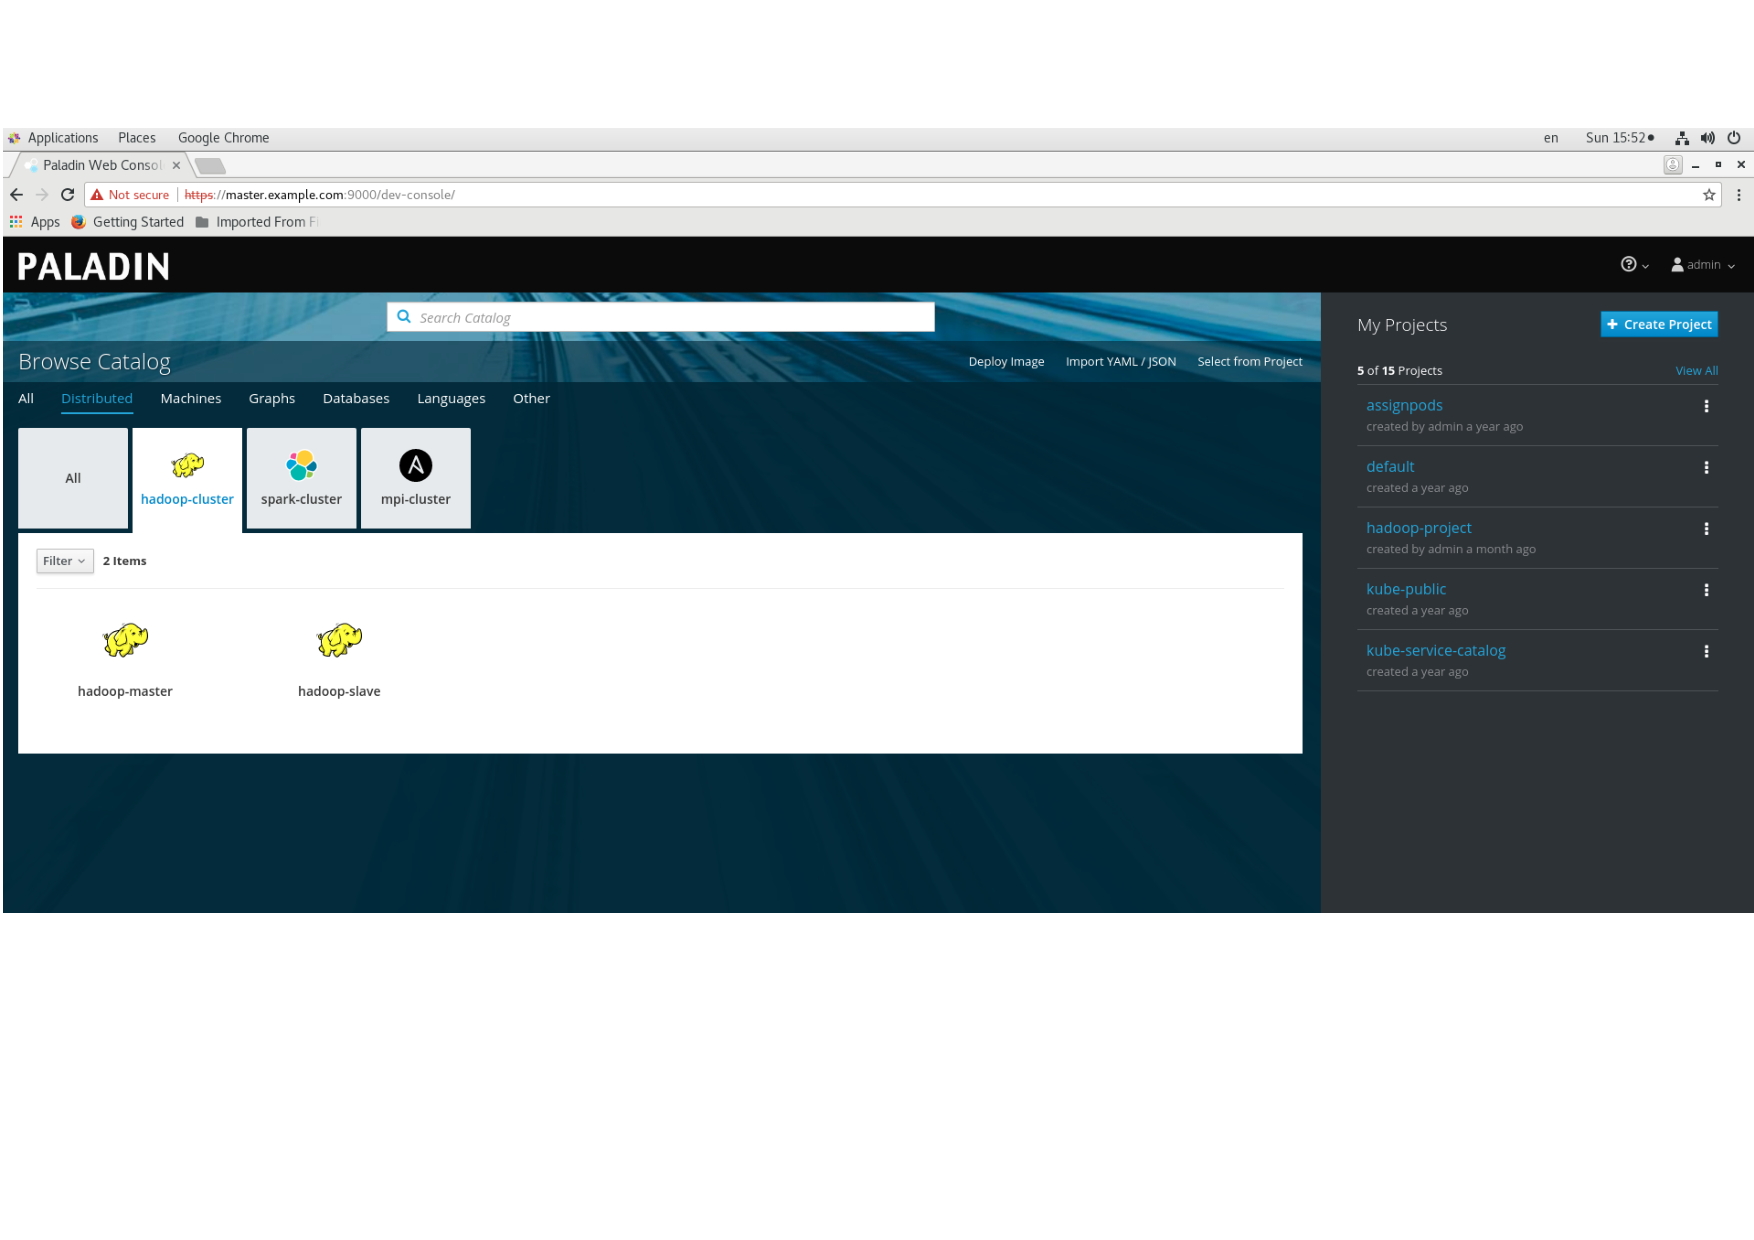
\includegraphics[width=13cm, height=7cm]{origin-web-console}
	\caption{Paladin数据处理框架部署服务}
\end{figure}

至此,整个Paladin大数据存储管理和计算框架快速部署容器云平台部署完成,实现了存储计算分离,用户既能进行大数据存储管理,实现普通的云存储系统,又能快速构建大数据处理容器应用框架,实现海量数据处理,为普通用户提供优秀的大数据容器云配套服务。

\section{多计算框架容器应用开发}
在构建分布式计算应用时,容器数量动态增减变化时需要能自动发现其数量的变化,并自动搭建好计算环境。如在Hadoop容器应用计算框架下,有10个计算容器,减少4个后,应用框架要能够快速发现并自动缩减为6个容器应用的Hadoop计算环境。因此,分布式计算框架容器应用中需要内嵌一个服务自发现组件,当前分布式有Zookeeper、Etcd、Serf等,本文用Serf做服务注册和自发现组件。

\subsection{Serf服务发现}
在分布式计算框架中,有的计算框架是主从结构如Hadoop、Spark等,有的只是简单的计算框架如MPI等,因此需要一个去中心化的服务发现方案。HashCorp开源的Serf是一个去中心化的服务发现和编排项目,具有成员管理、服务检测、高可用、分区容错等功能,是一个轻量级的服务组件。Serf底层实现Gossip协议,一种类似病毒感染的传播协议,能够快速自动感知节点上线和下线。构成分布式计算框架中的容器应用上都维护一个成员列表,并将节点列表随机发送给周围节点,发送方式有Push和Pull两种,即主动发送和被动请求方式。Serf有一个时效检测器,定期轮询节点列表,给列表中的节点发送心跳包,确保所有的节点在线。

Serf在分布式处理框架的每个应用容器上运行一个serf agent,在第一个容器应用上创建一个聚簇,后面创建容器的代理将会自动连接已存在的聚簇,形成一个集群。Serf是一个去中心化的服务方案,没有一个集中注册的节点,是一个弱一致性的方案,但具有较高的可用性和容错性。在常见的中心化集群中,集群的状态由master维护,通常为了可靠性需要双备份甚至多备份主节点,主节点往往是整个集群的性能瓶颈。在集群规模较大时,信息的传播给网络带来巨大的负载,集群的管理效率和正确性受到挑战,集群规模往往有一个上限。去中心化的集群可以进行大规模扩展,其效率和可靠性几乎不受集群规模的影响,Kubernetes底层用Etcd做服务发现,其规模上限通常在一万左右,而Docker Swarm底层用serf,其规模可以更大,Kubernetes的Etcd将会是制约其集群规模上限的重要因素。

Serf从功能上而言,自下而上可以分为三层:Gossip协议层、消息中间件、客户端接口。Gossip协议层封装Gossip协议以及集群管理的相关操作;消息中间件对传播消息进行封装,包括管理的消息、UserEvent、Query等各种处理逻辑,其中UserEvent是一个单向无需应答的消息,Query是需要应答的双向消息;客户端接口处理集群的输出输出格式,提供rpc接口。Serf是一个弱一致性的解决方案,让节点之间直接进行信息交流,提升软件平台服务自主性,是一个简单、高效、可靠的去中心集群管理和服务发现系统实现。

\subsection{Hadoop计算框架开发}
在Paldin容器云平台计算框架部分,需要开发多种分布式处理框架,方便用户快速构建大数据处理环境。用户通过web-console与平台进行交互,只需通过鼠标操作就能构建所需的计算环境和配置容器资源,实现快速自动化部署。计算框架最终以模板Template存在集群中,所需的镜像文件在Docker私有仓库registry中,所有用户都重复使用该模板,其构建过程如下所示。
\begin{figure}[H] % use float package if you want it here
	\centering
	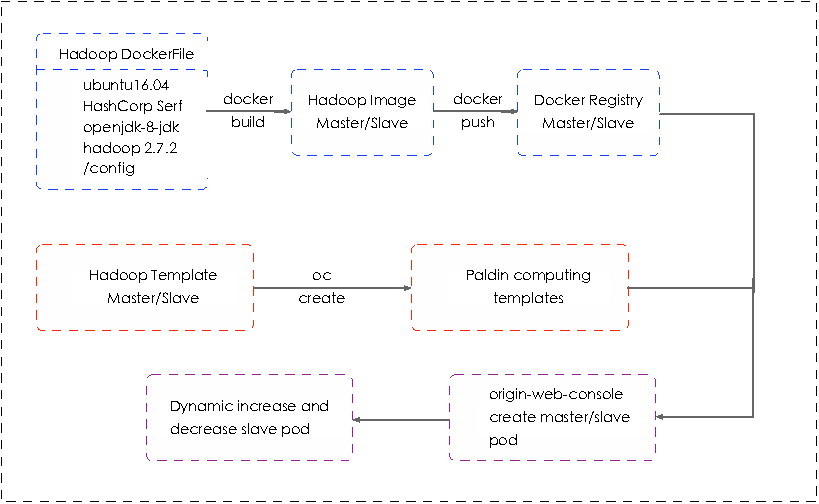
\includegraphics{hadoop-flow}
	\caption{Hadoop容器处理框架开发流程图}
\end{figure}

首先构建Hadoop环境容器应用的镜像文件,编写Hadoop Master和Slave的DockerFile文件,该文件在操作系统镜像ubuntu16.04的基础上安装Hadoop所需的环境,主要包括openjdk-8-jdk、hadoop-2.7.2、wget等,用于配置免密dnsmasq、openssh-server以及服务自发现Serf,将Hadoop所需的配置文件一并修改,整体打包成镜像,部分DockerFile源码如下:
\begin{lstlisting}[ language=csh]
FROM ubuntu:16.04
MAINTAINER gongkunjxl <gongkunjxl@163.com>
RUN sed -i 's/archive.ubuntu.com/mirrors.ustc.edu.cn/g' /etc/apt/sources.list
RUN apt-get install -y unzip curl dnsmasq openssh-server
RUN apt-get install wget vim openjdk-7-jdk fuse libglib2.0-0
# dnsmasq configuration
ADD dnsmasq/* /etc/
# install serf
RUN curl -Lso serf.zip https://releases.hashicorp.com/serf/0.5.0/serf_0.5.0_linux_amd64.zip
RUN unzip serf.zip -d /bin 
RUN rm serf.zip
#ADD hadoop-2.7.2.tar.gz /root/
RUN wget XXX/hadoop-2.7.2.tar.gz(根据实际需要选择版本)
RUN tar -xzvf hadoop-2.7.2.tar.gz
RUN mv hadoop-2.7.2 /usr/local/hadoop
RUN rm hadoop-2.7.2.tar.gz
\end{lstlisting}

此外,还有一些修改的配置文件和样例文件,以及paladin-client挂在文件系统的客户端等,使用docker build命令全部打包成容器Image文件,将文件push到私有仓库中,平台私有仓库的Ip为172.30.7.23:5000,在以后的template文件中将使用该镜像文件源。为重复使用该镜像文件以及用户通过web-console快速构建Hadoop计算框架,需要做成模板放置在平台上,其模板小部分代码如下:
\begin{lstlisting}[ language=csh]
{
"kind": "Template",
"apiVersion": "v1",
"metadata": {
"name": "hadoop-master",
"annotations": {
"description": "Hadoop Master",
"iconClass": "icon-hadoop",
"tags": "hadoop"
}
 "objects": [
{
"kind": "Service",
"apiVersion": "v1",
"metadata": {
"name": "${APP_SERVICE_NAME}",
},
.......
\end{lstlisting}

该模板包含一个Service、一个DeploymentConfig,部署弯沉过后可以实现Container的自动伸缩。根据容器编排引擎Kubernetes底层网络原理,两个Pod之间可以实现直接IP互相访问,同一个Namespace下的Pod可以通过网桥直接通信。为了更好的实现对外服务,Pod的Service服务将其IP地址内嵌到后来创建的同一Namespace下的所有Pod中,但在创建Service之前的Pod中不会嵌入IP,这是实现Pod构成集群的最好方式。利用网络管理的这一特性,使用Serf对第一个容器应用创建聚簇,后面容器的Serf代理通过第一个容器的内嵌IP实现集群发现服务。如第一个容器应用是hadoop-master,由于其创建了Service服务,后面创建的所有hadoop-slave容器中都会有\$HADOOP\_MASTER\_SERVICE\_HOST环境变量为hadoop-master的IP地址,实现集群的构建。通过web-console可以快速构建Hadoop处理环境,并根据资源需求实现容器的自动伸缩,按需配置服务。
\begin{figure}[H] % use float package if you want it here
	\centering
	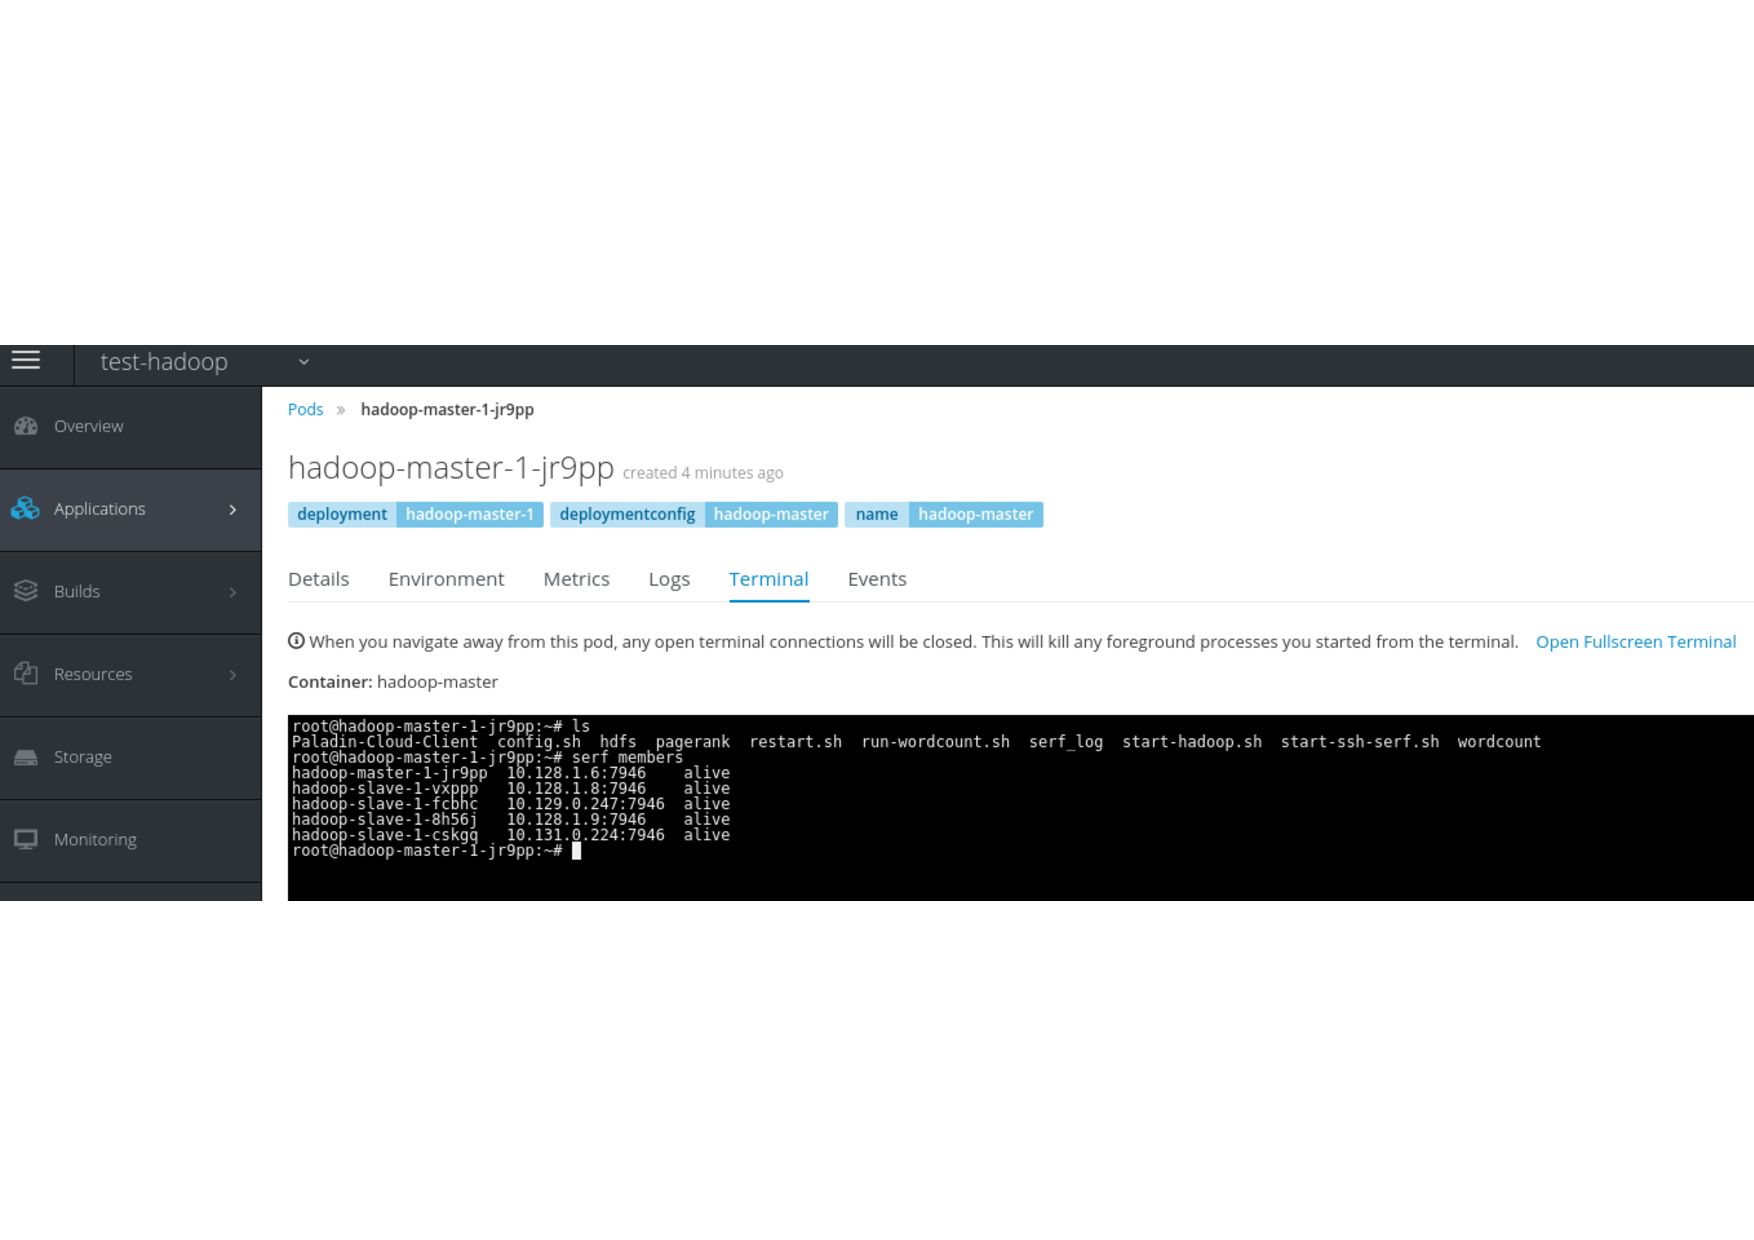
\includegraphics[width=13cm, height=5cm]{hadoop-member}
	\caption{Hadoop集群成员}
\end{figure}

同样可以通过hadoop-master Pod的IP地址进行访问,在浏览器中访问Pod的50070和8088端口,查看Hadoop集群状态和运行任务:
\begin{figure}[H] % use float package if you want it here
	\centering
	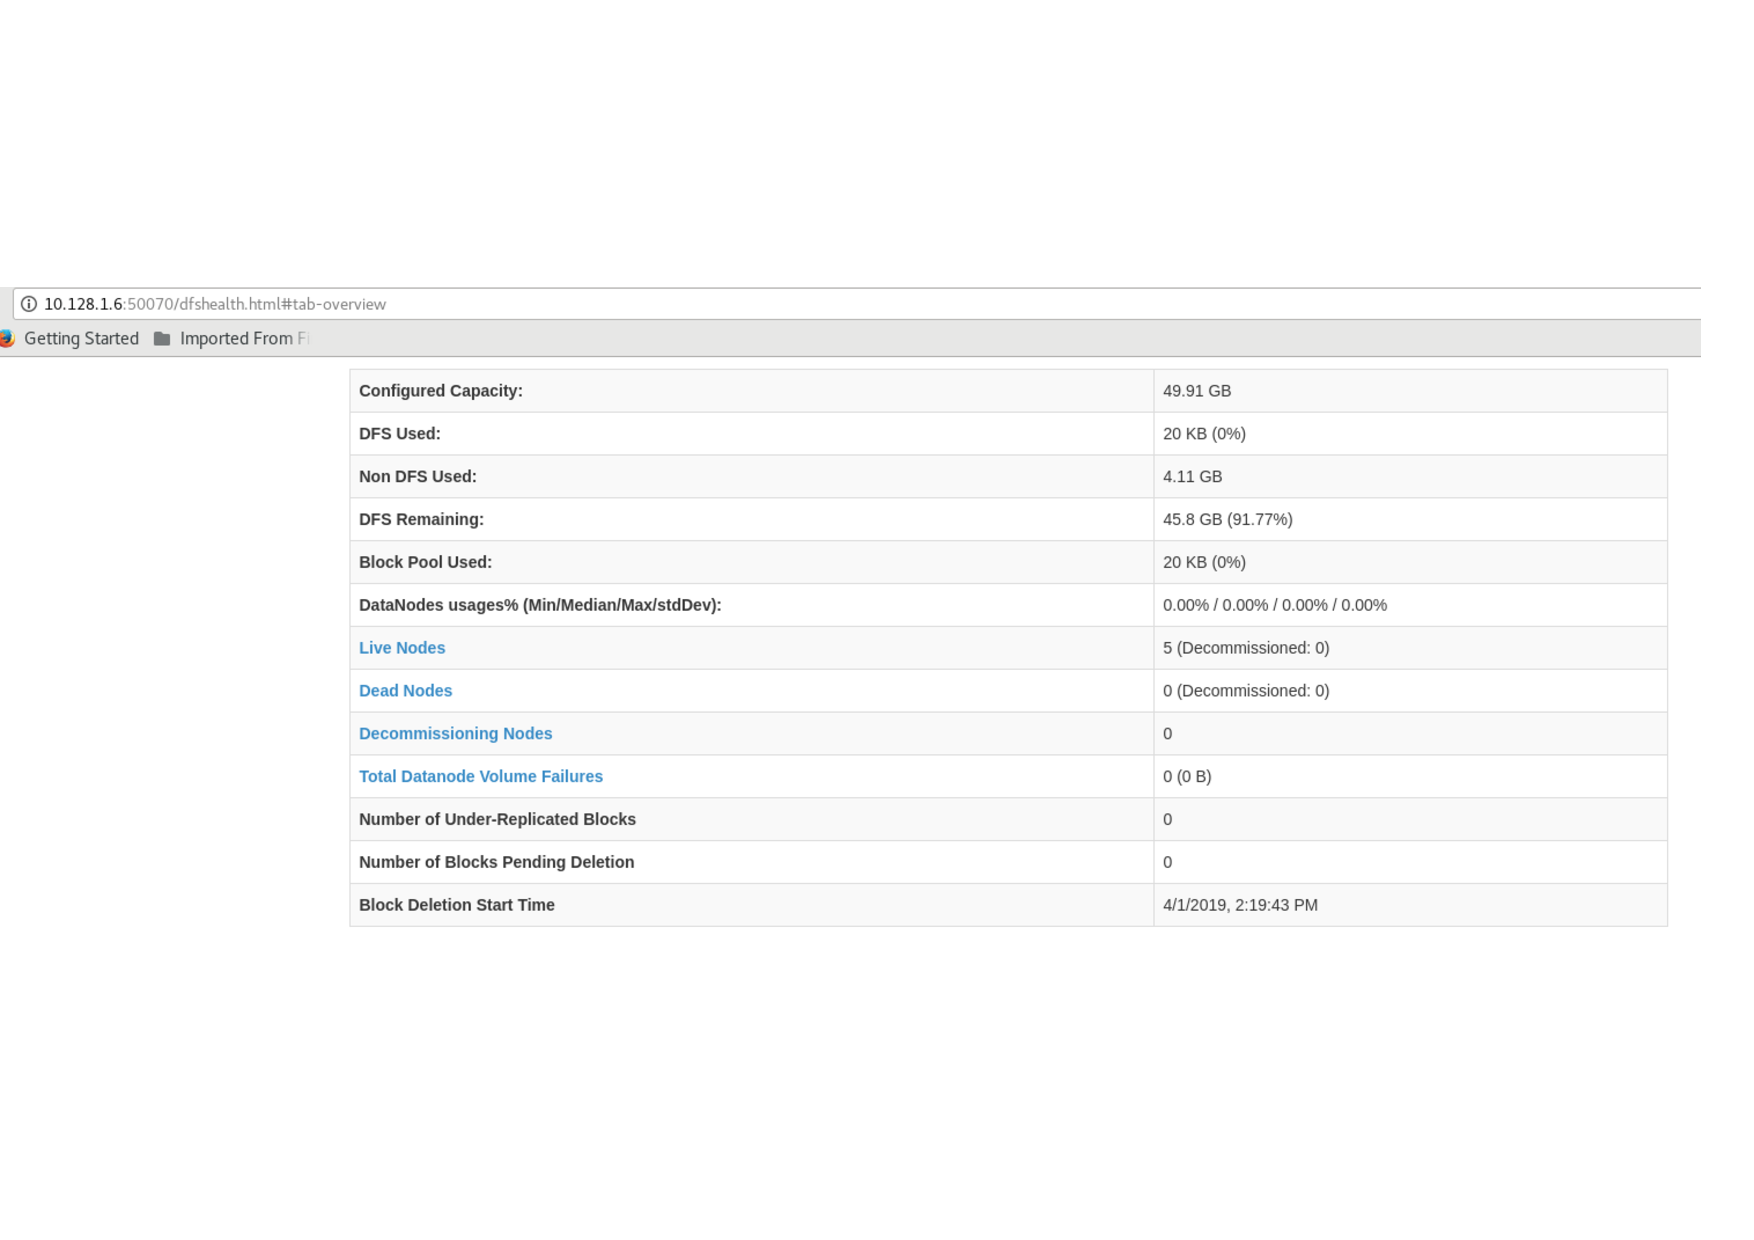
\includegraphics[width=13cm, height=5cm]{hadoop-status}
	\caption{Hadoop集群状态信息}
\end{figure}
在构建的Hadoop集群上运行wordcount样例,通过8088端口查看任务信息:
\begin{figure}[H] % use float package if you want it here
	\centering
	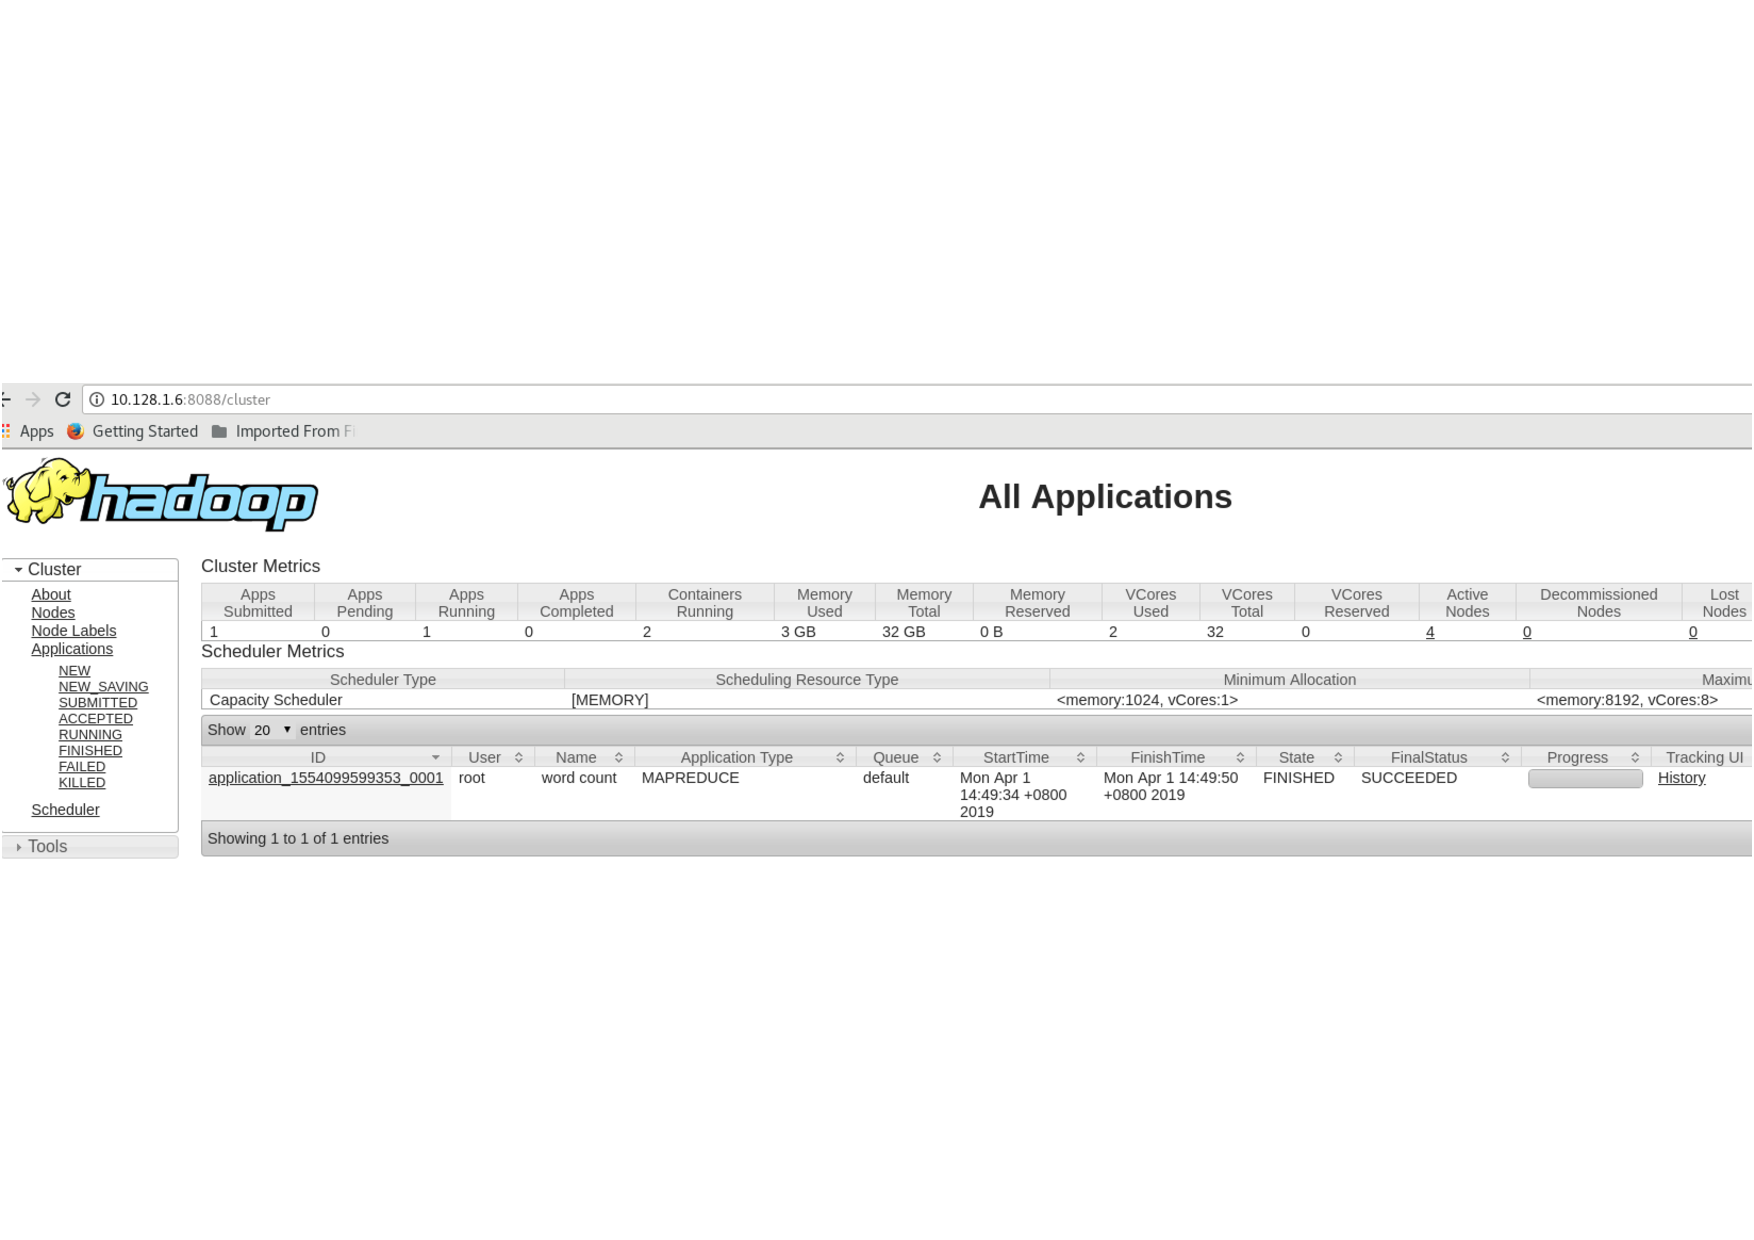
\includegraphics[width=13cm, height=5cm]{hadoop-task}
	\caption{Hadoop任务状态信息}
\end{figure}

至此,一个完整Hadoop容器应用处理框架构建完成,用户可以非常方便的在web-console上实现Hadoop环境的快速部署,并根据资源需求动态伸缩Pod数量,实现容器云平台的按需服务,并通过web查看器任务和集群状态。

\subsection{其他计算框架开发}
上一小节详细介绍了Paladin平台上Hadoop分布式处理框架的开发流程,使用上述的开发流程,构建其他的数据处理框架。原始的Docker hub中镜像文件大多只支持单个容器应用,即一个容器机器复制,比如PHP、Go、Java、Ruby、Python等语言类容器应用,以及Mysql、MongoDB、MariaDB等数据存储类容器。多分布式的数据处理框架和计算框架几乎没有,因此我们开发了离线数据批处理Hadoop、Spark、流计算Storm、Flink、分布式MPI、机器学习框架Mahout、Tensorflow、图计算系统GridGraph、Regraph等。众多的分布式处理可以满足绝大部分用户的需求,使得该平台将大数据存储管理和数据处理框架有机集合,并实现存储计算分离。底层基于Docker容器应用,集群整体的性能比虚拟机要优秀,减少了虚拟机系统隔离的开销。该平台上构建的分布式模板如下:
\begin{figure}[H] % use float package if you want it here
	\centering
	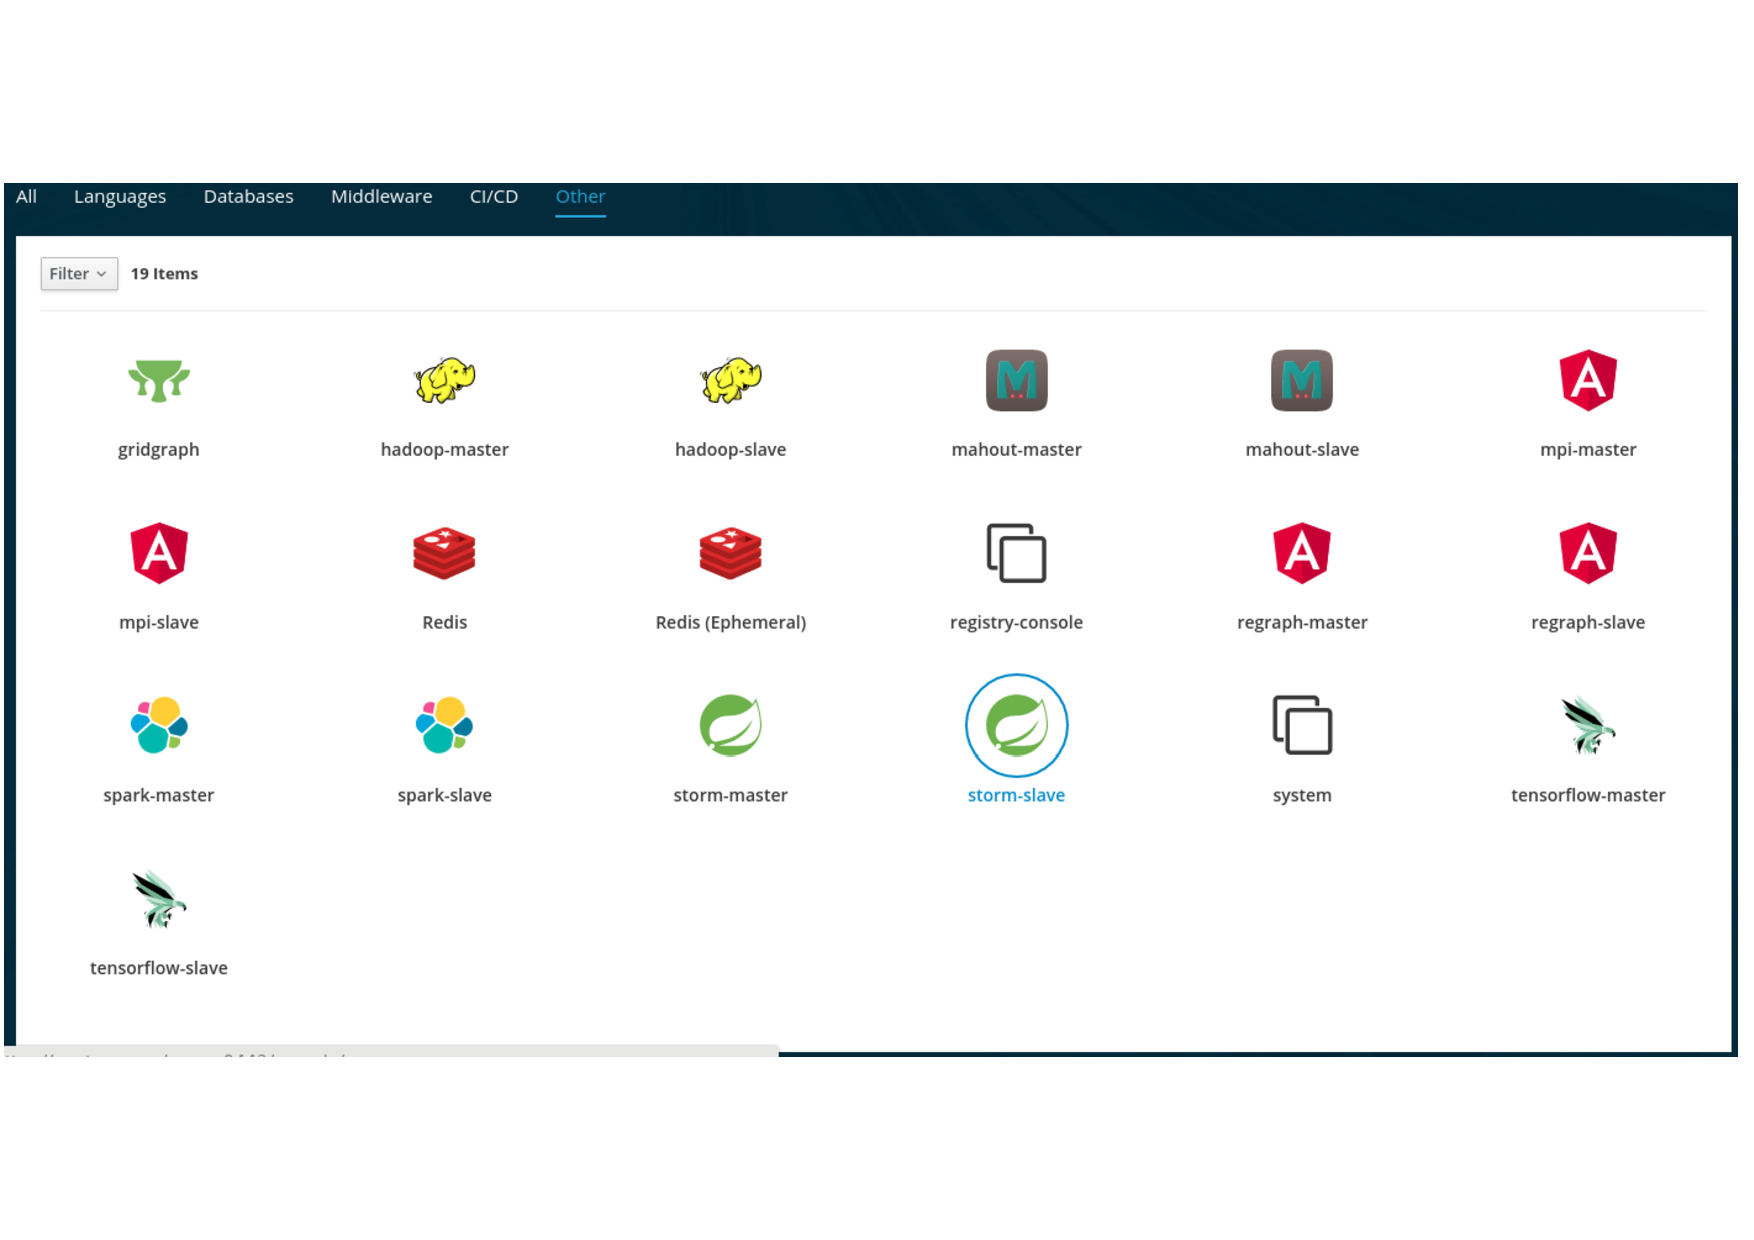
\includegraphics[width=13cm, height=7cm]{paladin-distribute}
	\caption{Paladin平台支持的处理框架模板}
\end{figure}

用户选择需要构建的处理框架,创建其第一个容器应用及其Service,容器应用内部的Serf同时创建集簇,后创建的容器应用通过Service提供的IP用其Serf代理自动连接集簇,构建一个集群。根据实际的资源需求,用户动态调整Pod数量,伸缩其资源,实现按需服务。容器应用中的Serf代理会自动监控容器应用的伸缩,用户调整完Pod数量后无需重启或重新连接集群,Serf服务发现解决方案很好解决分布式框架容器应用上线下线问题。Paladin平台给用户提供了一个web-console的可视化服务,用户无需了解部署原理和细节,甚至无需关心其构建过程,只需要根据实际需要配置处理框架的容器数量,几秒钟内就可以搭建好开发测试环境。用户把所有的精力集中在应用的开发生,完全从集群和环境配置中解放出来。该平台同时还提供数据存储管理可视化,可以挂载到所有的容器应用中,无需用户手动管理和数据节点分配,全自动化的存储计算分离。

\section{多计算框架应用下MRWS性能测试}
搭建完容器云数据管理存储和多计算框架容器应用环境快速构建平台后,需要对MRWS调度性能进行测试,对比MRWS、Kubernetes、Random、FirstFit四种调度算法的性能。由于是小规模的容器云集群,无法对资源利用率进行大规模测试,大规模的仿真在ContainerCloudSim已经完成,因此只进行多计算框架容器应用混合部署下几种调度方案的性能。

\subsection{混合部署多计算框架}
Paladin平台只有五个实际的物理的节点,要在此小规模的集群上测试四种算法的性能,不能进行大规模的负载模拟。因此,构建集中较为典型的密集型应用容器,通过密集型应用的样例运行时间测试集中算法的优劣。Hadoop作为离线数据批处理,在海量数据处理map阶段完成后不能将所有的数据都放入内存做shuffle,要写入磁盘,其处理数据的方式大部分应用都是I/O密集型应用,因此用其数据读写样例作为I/O密集型容器应用,即Hadoop框架作为I/O密集型调度用例。Spark处理框架的特点是将大部分数据放入内存运算,每次将map输出的结果保存在内存中,大部分应用是内存密集型应用,因此Spark的PageRank计算用作内存密集型应用。MPI多用于分布式计算,网络和计算资源通常是其瓶颈,在MPI的pi计算是一种CPU密集型应用,因此用作调度测试用例。Paladin集群上将混合部署Hadoop、Spark和MPI三种多计算框架,每个计算框架的容器数量相同,Hadoop上运行I/O和网络密集型应用TestDFSIO.java、Spark上运行内存密集型应用支持向量机PageRank、MPI上运行CPU密集型应用PI计算。
\begin{table}[H]
	\centering\dawu[1.3]
	\caption{用于调度算法测试的计算框架}
	\begin{tabular}{|p{2cm}<{\centering}|p{2cm}<{\centering}|p{2cm}<{\centering}|p{2cm}<{\centering}|} \hline
		框架类型 & 类型 & 运行程序 & 容器数量 \\ \hline
		MPI & CPU密集 & PI计算 & 15 \\ \hline
		Spark & 内存密集 & PageRank & 15  \\ \hline
		Hadoop & I/O密集 & TestDFSIO & 15  \\ \hline
	\end{tabular}
\end{table}

调度算法的开发,Paladin是基于OpenShift Origin搭建的,OpenShift Origin是一个开源的容器云平台,其底层的容器编排引擎是Kubernetes。该平台只是搭建与Kubernetes上,并未修改其源码,因此开发该平台的调度方式和Kubernetes开发调度算法完全一样,最后只需要将调度算法的名称注册到平台的配置文件origin-master.conf中即可替代原有的算法。虽然Kubernetes提供了大量的API,但其使用较为繁琐,整个引擎的语言都是go开发,因此使用client-go进行快速开发。client-go是调用Kubernetes集群资源的客户端,对Kubernetes前置的API封装的二次开发都使用client-go这个第三方包实现,可以对集群资源对象进行增删查改。因此,四种调度算法也是使用client-go第三方包开发完成,实现与集群的交互。

进行调度算法测试前,需要构建三种计算框架的容器应用,并对容器应用进行资源配置。根据其运行应用的类型,在相应维度上进行适当对配置,CPU密集型容器应用对CPU资源多配置,其他维度相对配置较少。为了测试混合部署的集群性能,不设置容器的资源使用上限,设置其资源使用下限,目的在于容器应用可以快速完成任务。如一个容器CPU限制使用30\%,如果物理节点上只存在一个容器,则该容器可以使用全部的CPU资源。主要在于测试多计算框架混合部署的场景下,几种调度算法对容器应用进行调度,整个集群完成全部计算框架处理任务的时间,该时间用于衡量集群性能,也就是调度算法的优劣。
\begin{table}[H]
	\centering\dawu[1.3]
	\caption{Random调度算法应用容器分布}
	\begin{tabular}{|p{2cm}<{\centering}|p{1.8cm}<{\centering}|p{1.8cm}<{\centering}|p{1.8cm}<{\centering}|p{1.8cm}<{\centering}|p{1.8cm}<{\centering}|} \hline
		\diagbox[innerwidth=1.8cm]{类型}{节点} & Master & Node1 & Node2 & Node3 & Node4 \\ \hline
		MPI-pod & 3 & 5 & 2 & 4 & 1 \\ \hline
		Spark-pod &3 & 2 & 3 & 2 & 5 \\ \hline
		Hadoop-pod & 1 & 4 & 5 & 2 &3 \\ \hline
		Total & 7 & 11 & 10 & 8 & 9 \\ \hline
	\end{tabular}
\end{table}
\begin{table}[H]
	\centering\dawu[1.3]
	\caption{FirstFit调度算法应用容器分布}
	\begin{tabular}{|p{2cm}<{\centering}|p{1.8cm}<{\centering}|p{1.8cm}<{\centering}|p{1.8cm}<{\centering}|p{1.8cm}<{\centering}|p{1.8cm}<{\centering}|} \hline
		\diagbox[innerwidth=1.8cm]{类型}{节点} & Master & Node1 & Node2 & Node3 & Node4 \\ \hline
		MPI-pod & 5 & 2 & 5 & 2 & 1 \\ \hline
		Spark-pod & 3 & 6 & 1 & 5 & 1 \\ \hline
		Hadoop-pod & 2 & 5 & 3 & 5 & 1 \\ \hline
		Total & 10 & 13 & 9 & 12 & 3 \\ \hline
	\end{tabular}
\end{table}
\begin{table}[H]
	\centering\dawu[1.3]
	\caption{Kubernetes调度算法应用容器分布}
	\begin{tabular}{|p{2cm}<{\centering}|p{1.8cm}<{\centering}|p{1.8cm}<{\centering}|p{1.8cm}<{\centering}|p{1.8cm}<{\centering}|p{1.8cm}<{\centering}|} \hline
		\diagbox[innerwidth=1.8cm]{类型}{节点} & Master & Node1 & Node2 & Node3 & Node4 \\ \hline
		MPI-pod & 3 & 3 & 3 & 3 & 3 \\ \hline
		Spark-pod &3 & 3 & 3 & 4 & 2 \\ \hline
		Hadoop-pod & 1 & 3 & 5 & 1 & 5 \\ \hline
		Total & 7 & 9 & 9 & 8 & 10 \\ \hline
	\end{tabular}
\end{table}
\begin{table}[H]
	\centering\dawu[1.3]
	\caption{MRWS调度算法应用容器分布}
	\begin{tabular}{|p{2cm}<{\centering}|p{1.8cm}<{\centering}|p{1.8cm}<{\centering}|p{1.8cm}<{\centering}|p{1.8cm}<{\centering}|p{1.8cm}<{\centering}|} \hline
		\diagbox[innerwidth=1.8cm]{类型}{节点} & Master & Node1 & Node2 & Node3 & Node4 \\ \hline
		MPI-pod & 3 & 4 & 3 & 3 & 2 \\ \hline
		Spark-pod &2 & 4 & 3 & 3 & 3 \\ \hline
		Hadoop-pod & 3 & 2 & 3 & 3 & 4 \\ \hline
		Total & 8 & 10 & 9 & 9 & 9 \\ \hline
	\end{tabular}
\end{table}
根据四种调度方案容器应用的分布可以看出,Random随机调度三个计算框架的容器应用,不做任何的资源空闲率平衡,CPU密集型容器应用MPI-pod在Node1上有5个,而Node4上只有1个。I/O密集型容器应用Hadoop-pod在Master上有1个,但Node2上有5个,各种容器应用随机调度分配,但是整体的容器应用各节点上相差不大。这种调度方式必然会导致Node4上CPU资源紧缺,Node2上I/O资源紧缺,影响集群性能。FirstFit也不做资源使用率平衡,每次选择第一个满足资源的节点进行调度,导致前面的节点负载过高,后面节点负载较低,从整体容器应用分布来看,Node4上仅分配了三个容器应用,而Node1节点高达13个,导致部分节点各种资源负载过高,部分节点资源利用率不足。Kubernetes对CPU和内存的资源空闲率做了平衡,尽量使内存和CPU资源平衡使用,从分布看出CPU密集型MPI-pod和内存密集型Spark-pod在各节点上的分布较为均匀,都在$2\sim4$个容器应用,但是I/O密集型应用Hadoop-pod分布不均,Node1和Node3上只有1个容器应用,Node2和Node4上有5个容器应用,这种只注重CPU和内存均衡的调度方式导致集群各节点I/O密集型分布不均,影响集群性能。MRWS调度方式可以看到几种密集型应用分布较为均衡,各节点的各种密集型容器应用都在$2\sim4$个,整体节点容器数量也在$8\sim10$个之间。整个集群各维度资源利用率较为均衡,集群负载较好。

\subsection{单个计算框架服务性能}
针对四种调度方案的容器应用分布,首先进行单个计算框架的性能测试,在容器应用中设置资源的下限,不限制应用容器使用资源的量,在同一个节点上的容器应用可以自由竞争资源。对比几种调度算法单个计算框架应用执行的时间,在Hadoop-pod中进行TestDFSIO测试,分别读写15个128M的文件,记录总体时间,Spark-pod中进行PageRank程序计算,测试文件大小约3.2M,轮数为2000轮迭代,MPI-pod中进行pi运算,15个节点110000轮计算。每个调度算法分别运行三次,取三次运算结果的平均值,各计算框架容器应用执行时间如下(以秒为单位):
\begin{table}[H]
	\centering\dawu[1.3]
	\caption{四种调度算法应用容器执行时间}
	\begin{tabular}{|p{3cm}<{\centering}|p{3.5cm}<{\centering}|p{3cm}<{\centering}|p{2.5cm}<{\centering}|} \hline
		\diagbox[innerwidth=3cm]{调度}{容器应用} & Hadoop-TestDFSIO & Spark-PageRank & MPI-PI \\ \hline
		Random & 255.92 & 267.33 & 387.19  \\ \hline
		FirstFit & 276.48 & 274.67 & 390.69  \\ \hline
		Kubernetes & 250.44 & 252.00 & 214.42  \\ \hline
		MRWS & 228.33 & 250.52 & 212.88  \\ \hline
	\end{tabular}
\end{table}
对比四种调度算法单计算框架下容器应用的执行时间,可以很明显大发现在进行I/O密集型容器应用Hadoop-TestDFIO测试时,Random、FirstFit以及Kubernetes调度算法没有考虑I/O资源均衡利用,导致多个I/O密集型应用被调度到同一节点。在容器中运行应用程序时,大量I/O密集型应用竞争I/O和网络资源,导致程序效率低下,执行时间过长。MRWS调度方式考虑I/O和网络带宽因素,尽量分散到集群各几点上,其性能最佳,Hadoop-TestDFSIO执行时间最短,FirstFit效果最差,Random和Kubernetes相差不大。在单独运行内存密集型应用Spark-PageRank容器应用下,Random和FirstFit都不考虑内存利用率均衡性,其运行时间最长,尤其是FirstFit将大量内存密集型调度到了同一个节点,使得内存成为该节点瓶颈,运行时间最长。Random随机分配节点,其效果一般,Kubernetes和MRWS均做了内存利用率均衡,其效果较好,各内存密集型容器大致可以分散到集群各节点上,其效果最佳。与内存类似,CPU密集型应用表现最为明显,Pi运算是一个典型的计算密集型应用,大量的时间花费在三角函数的运算上,Random和FirstFit均不做CPU利用率均衡,导致大量的CPU密集型应用调度到同一个节点,该节点的CPU成为其瓶颈,运行时间较长。Kubernetes和MRWS调度可以将CPU密集型应用尽可能分散到各节点上,运行时间大大缩短。

以CPU密集型应用调度为例,普通用户并不关心容器应用被调度到集群的哪个节点,只在乎计算框架应用的执行时间最短。在分布式计算MPI-PI程序时,用户将任务分成15份发送到15个容器应用上进行PI运算,如果某个节点上部署的MPI-pod越多,该节点上CPU资源竞争压力越大,完成计算任务的时间越长。下面两图展示FirstFit和Kubernetes调度算法下集群中各节点CPU利用情况:
\begin{figure}[H] % use float package if you want it here
	\centering
	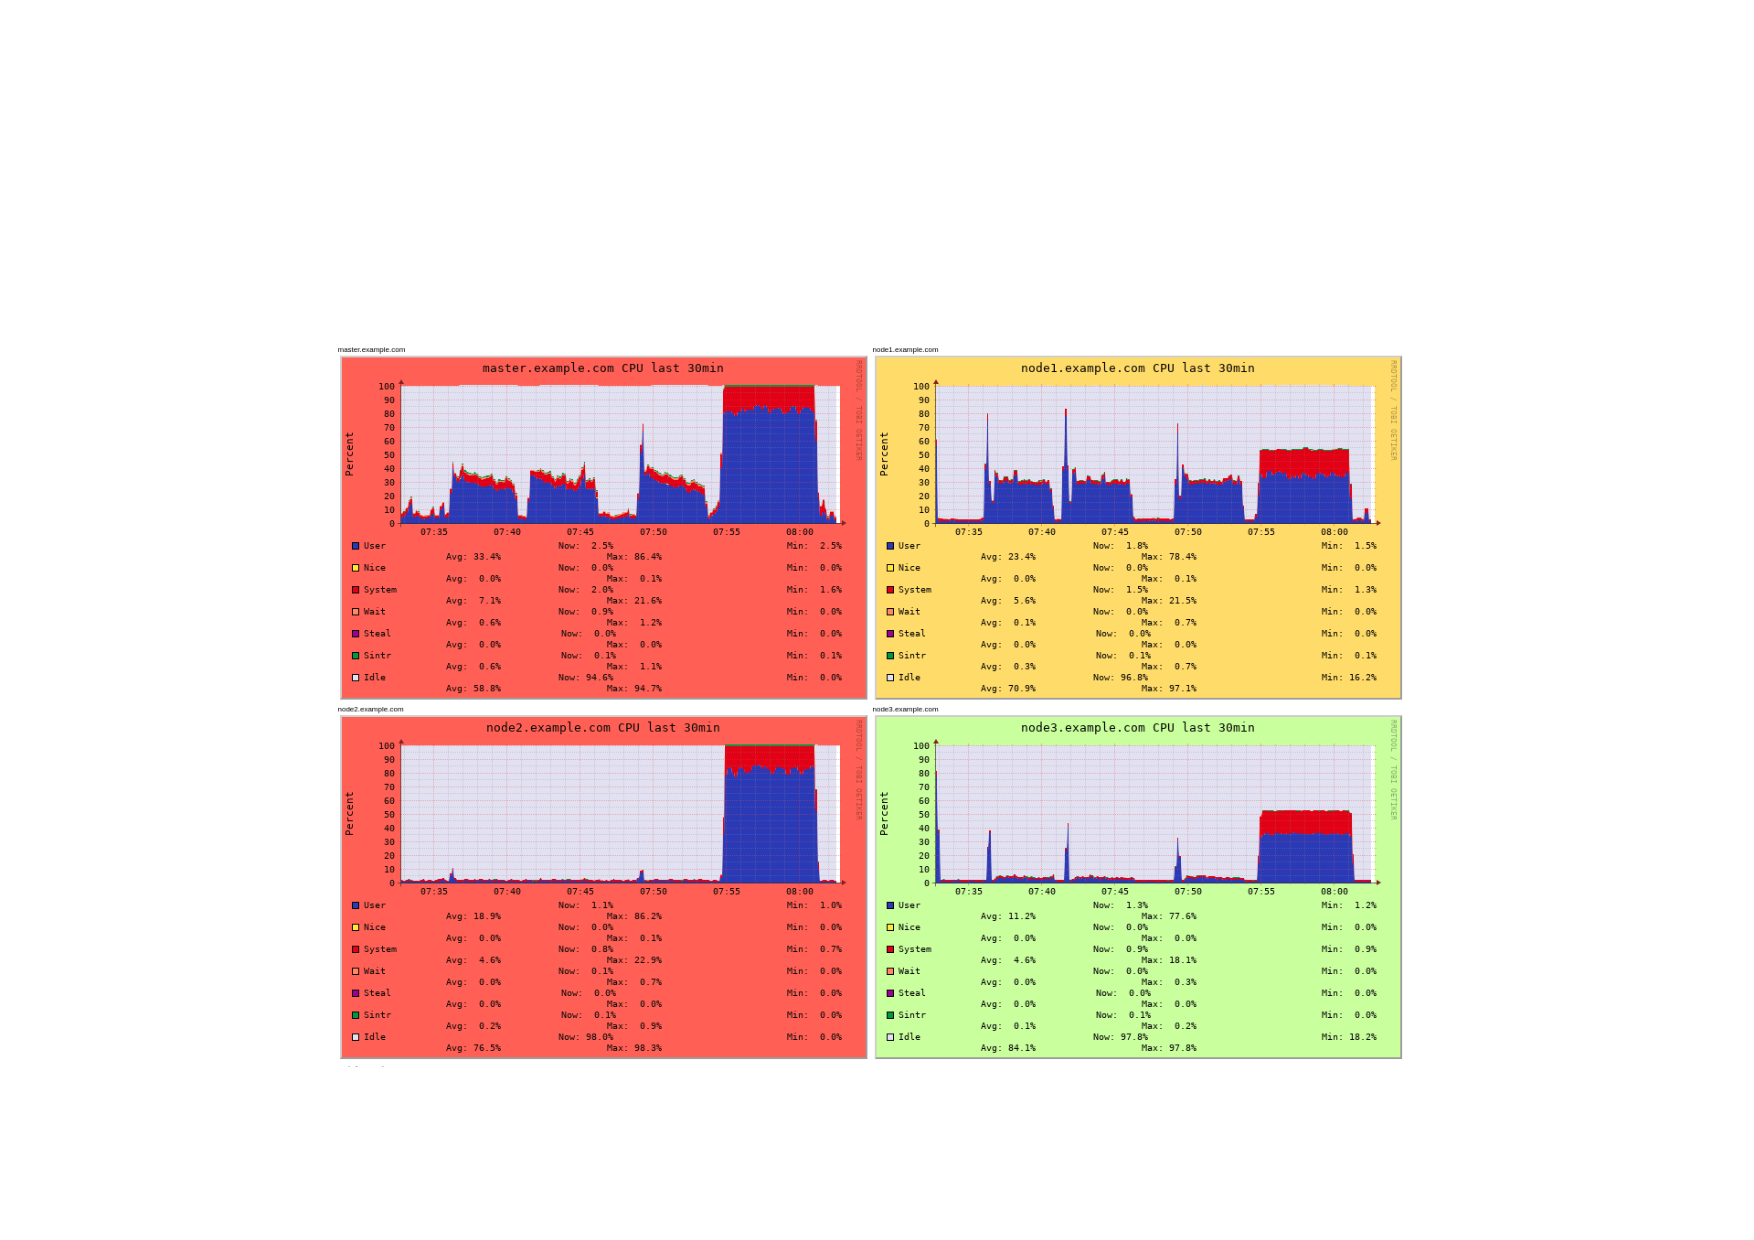
\includegraphics[width=13cm, height=7cm]{firstfit-cpu-utilization}
	\caption{FirstFit调度MPI-pod集群CPU利用情况}
\end{figure}
\begin{figure}[H] % use float package if you want it here
	\centering
	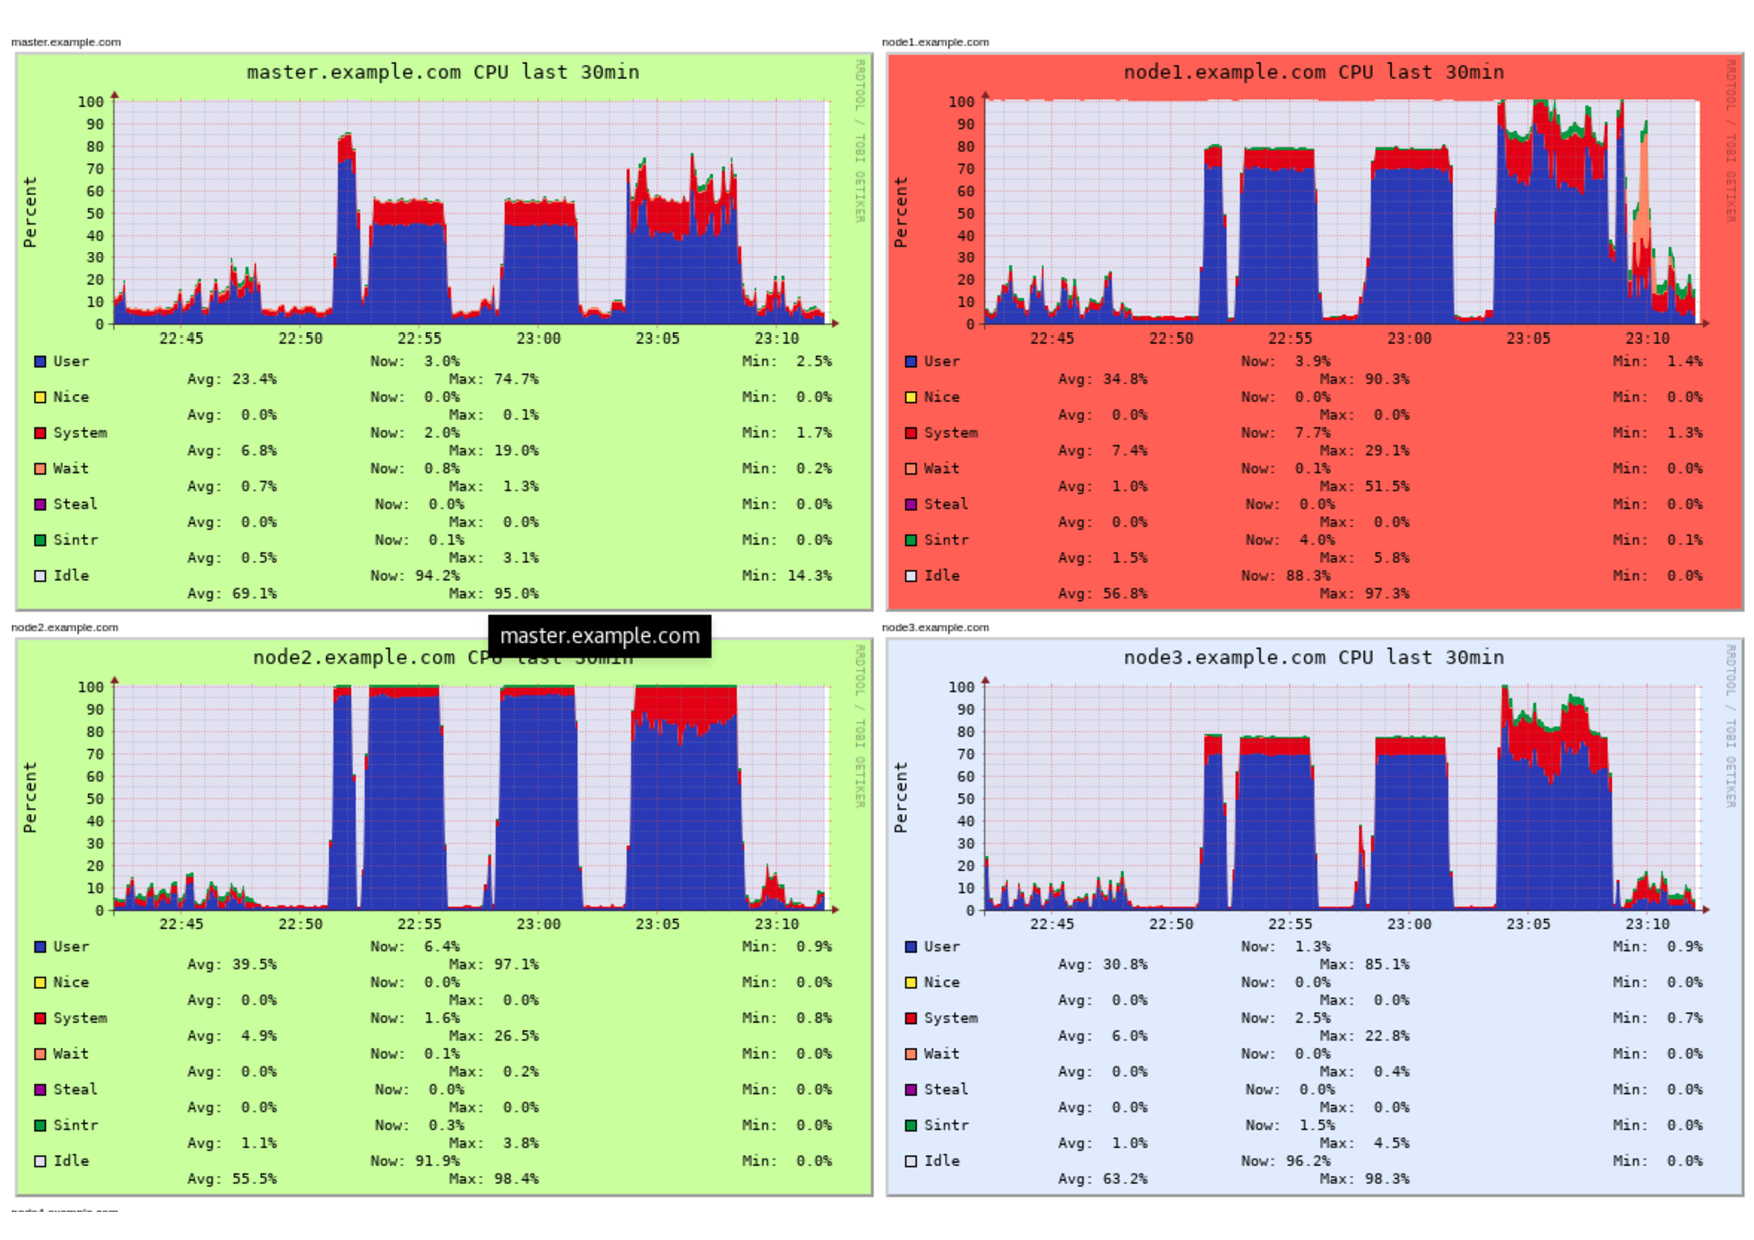
\includegraphics[width=13cm, height=7cm]{kubernetes-cpu-utilization}
	\caption{Kubernetes调度MPI-pod集群CPU利用情况}
\end{figure}
上述两图是在集群上部署Ganglia集群监控下两种调度算法的CPU利用率,可以很明显发现在FirstFit调度下Node3和Node4上的CPU利用不足,而Master和Node2上CPU竞争激烈,影响了MPI-PI计算框架下容器应用的执行时间,而Kubernetes调度下各节点CPU资源利用较为充分,执行时间较短。

\subsection{混合部署多计算框架下的服务性能}
混合部署三种密集型容器应用框架,同时运行Hadoop-TestDFSIO、Spark-PageRank和MPI-PI容器应用程序,对比几种调度算法的执行时间。混合部署和同时运行不同计算框架类似于多用户在容器云集群上部署运行不同的应用的场景,不仅相同密集型容器应用对节点上资源进行竞争,其他计算框架也会参与竞争资源。比如同一节点上MPI-pod对CPU进行竞争,该节点上部署的Spark-pod也会参与竞争CPU资源,调度不合理将导致整个集群性能低下,所有用户应用性能都将受到影响。每种调度算法执行3次,取3次执行时间的平均值,四种调度下同时运行多计算框架容器应用执行时间如下(秒为单位):
\begin{table}[H]
	\centering\dawu[1.3]
	\caption{同时执行多计算框架应用容器执行时间}
	\begin{tabular}{|p{3cm}<{\centering}|p{3.5cm}<{\centering}|p{3cm}<{\centering}|p{2.5cm}<{\centering}|} \hline
		\diagbox[innerwidth=3cm]{调度}{容器应用} & Hadoop-TestDFSIO & Spark-PageRank & MPI-PI \\ \hline
		Random & 316.46 & 584.00 & 418.43  \\ \hline
		FirstFit & 355.81 & 603.33 & 454.71  \\ \hline
		Kubernetes & 299.87 & 503.33 & 271.33  \\ \hline
		MRWS & 269.10 & 491.66 & 256.62  \\ \hline
	\end{tabular}
\end{table}
首先将执行时间和单个计算框架容器应用单独执行时间进行对比,在混合部署同时执行多计算框架下所有应用执行时间都变慢,如Hadoop-TestDFSIO在MRWS调度下单独执行时间是228.33,在混合部署执行下269.10,这是由于更多的容器容器应用参与资源竞争导致整体执行时间变慢。其中Spark-PageRank执行时间变化最为明显,这是由于PageRank的运算不仅需要大量的内存资源,还需要一定的CPU资源,而CPU资源被MPI-PI计算框架占用,导致其执行时间变慢。

对比各调度算法下混合部署多计算框架以及同时执行多计算框架容器应用执行时间,FirstFit性能最差,各计算框架执行时间最长,这是由于其每次选择第一个可用节点导致其资源利用不均,有的节点过载而有的节点资源利用不足。Random和Kubernetes相较于MRWS在Hadoop-pod的执行时间较差,整体而言MRWS调度算法西能你最优,各计算框架的执行时间相较于其他调度算法执行都最短。这是由于MRWS调度算法综合考虑了容器应用的CPU、内存、磁盘、网络带宽和节点已部署Pod的因素,利用FAHP自动建模和求解容器应用多维资源权重参数,采用空闲资源和资源利用均衡共同进行评分,选取最优的节点作为容器应用调度目标。这种调度方式在多计算框架下性能表现最为明显,通常在用计算框架处理大数据时Hadoop进行MapReduce时需要大量I/O,Spark是内存式的需要大量内存资源,MPI则用于计算密集型较多等。每个大数据处理框架都有自己相应的特点,在混合部署时需要充分考虑个计算框架的特点才能充分利用容器集群资源,实现多种密集型应用在节点上混合部署,提升集群服务性能。

\section{本章小结}
本章从实验的角度对比四种调度算法性能优劣,首先详细介绍云计算仿真平台CloudSim和容器云仿真平台ContainerCloudSim,在该平台上开发四种调度算法并进行大规模调度仿真,对比几种调度方法在集群资源利用和负载均衡方面的性能。通过对比分析,MRWS调度相较于其他几种调度方法无论在单节点各维度资源利用方面还是集群整体资源利用方面其负载均衡性较好,集群资源利用率也更高。然后介绍和部署实验室研发的大数据存储与处理容器云平台,这是一个存储与计算分离的容器云平台,平台主要用于大数据存储和处理。接着在该平台上开发数十种大数据处理框架,并以Hadoop批处理框架为例详细介绍其开发流程,用户通过origin-web-console与平台进行交互,在几秒钟之内快速构建大数据处理框架并进行容器伸缩扩展。最后,在Paladin平台进行多计算框架容器应用调度分析,对比几种调度算法下多计算框架容器应用的执行性能。分别以I/O和网络密集型应用Hadoop-TestDFSIO、内存密集型应用Spark-PageRank和CPU密集型应用MPI-PI计算框架容器应用为例,在混合部署几个计算框架时单独执行和同时运行下,对比各容器应用的执行时间,从而获取几种调度算法下集群的服务性能。



















